% ==========================================
% LatexRefinement Step Output: step4-05-05-25-tuesday-all-offset-final.tex
% Model: gemini-3.5-flash
% Temperature: 0.36
% TopP: 0.95
% TopK: 40
% MaxOutputTokens: 65535
% ThinkingBudget: 32768
% ThinkingLevel: HIGH
% Prompt Tokens: 38'456
% Candidates Tokens: 27'090 (inkl. Thinking Tokens)
% Cached Tokens: 0
% Processed on: 2026-07-10 13:49:53
% ==========================================

\lecturechapter{Dienstag}{5. Mai}{5. Mai 2026}{Graphentheorie}

\begin{nice-box}[Syllabus / Agenda]
In dieser Vorlesung beschäftigen wir uns mit den folgenden zentralen Themen der Graphentheorie:
\begin{itemize}
    \item \textbf{Das Handschlaglemma:} Formulierung, Beweis und alltägliche Interpretation.
    \item \textbf{Euler-Linien und Euler-Graphen:} Der Satz von Euler, das Königsberger Brückenproblem und das Dominoproblem als praktische Anwendung.
    \item \textbf{Hamilton-Kreise und Hamilton-Graphen:} Definition, Beispiele (platonische Körper, Hyperwürfel) und die Konstruktion von Gray-Codes.
    \item \textbf{Bipartite Graphen:} Definition, Zwei-Färbbarkeit und Nachbarschaften.
    \item \textbf{Der Heiratssatz von Hall:} Formulierung, Interpretation und ein vollständiger Induktionsbeweis.
\end{itemize}
\end{nice-box}

\section{Das Handschlaglemma}

\begin{spoken-clean}[00:00:00 - 00:01:58]
Hallo zusammen, wir fangen an. Herzlich willkommen zur elften Woche. Wir sind noch mittendrin in der Graphentheorie --- also ein ganz kleiner Einblick in das, worum es in einem Teil der Graphentheorie geht. Letzte Woche haben wir noch kurz mit einem Lemma aufgehört. Ich wollte das noch kurz umformulieren. 

Dieses Lemma heißt auch das Handschlaglemma. Das Schöne an der Graphentheorie ist: Man kann es oft so in alltägliche Situationen umformen --- oder viele Sachen sind vielleicht auch Probleme aus dem realen Leben ---, und dann kann man auf einmal sehen: Ah, das ist einfach ein Graph, und dann kann man das mit irgendeinem graphentheoretischen Lemma lösen. 

Das Handschlaglemma sagt, dass auf einer Party mit $n$ Gästen die Anzahl der Gäste, die einer ungeraden Anzahl von Personen die Hand geben, gerade ist. Und das war im Prinzip genau das, was wir am Ende der letzten Stunde bewiesen haben.
\end{spoken-clean}

\begin{math-stroke}
\begin{lemma}[Handschlaglemma]\label[lemma]{lem:handschlaglemma}
Auf einer Party mit $n$ Gästen ist die Anzahl der Gäste, die einer ungeraden Anzahl von Gästen die Hand geben, gerade.
\end{lemma}
\end{math-stroke}

\begin{proof}[Beweis des Handschlaglemmas]
\begin{spoken-clean}[00:01:58 - 00:03:38]
Der Beweis geht so: Wir betrachten einfach den Graphen $G = (V, E)$. Dabei ist $V$ genau die Menge der Gäste, und $E$ --- da es ein ungerichteter Graph ist --- sind einfach die Paare von Gästen, die sich die Hand geben. Und wir haben gesehen, dass die Anzahl der Knoten $x \in V$, deren Grad ungerade ist, immer gerade ist. 

Wir gehen natürlich davon aus, dass sich die Leute nicht selbst die Hand schütteln. Das geht nicht. Oder wenn man sich selbst die Hand schüttelt, dann zählt das wie zweimal Händeschütteln, weil man sich ja selbst quasi die Hand geschüttelt hat. Das machen wir also nicht. Das wollte ich einfach noch erwähnen, dass das der Fall ist. Gut, das dient einfach dazu, sich eine konkrete Situation für gewisse Resultate vorzustellen.
\end{spoken-clean}

\begin{math-stroke}
Betrachte den ungerichteten Graphen $G = (V, E)$, wobei:
\begin{itemize}
    \item \textbf{V:} $V := \{\text{Gäste}\}$
    \item \textbf{E:} $E := \{\{x, y\} \mid x \text{ und } y \text{ geben sich die Hand}\}$
\end{itemize}
Aus dem allgemeinen Handschlaglemma für Graphen wissen wir, dass die Summe der Grade aller Knoten stets gerade ist:
\[
\sum_{v \in V} \deg(v) = 2|E|
\]
Daraus folgt unmittelbar, dass die Anzahl der Knoten mit ungeradem Grad gerade sein muss:
\[
\left| \bigl\{ z \in V \;\big|\; \deg(z) \text{ ist ungerade} \bigr\} \right| \equiv 0 \pmod 2
\]
\end{math-stroke}
\end{proof}

\section{Euler-Linien und Euler-Graphen}

\begin{spoken-clean}[00:03:38 - 00:05:40]
Das Letzte, wofür wir letzte Woche leider keine Zeit mehr hatten, war diese Sache mit den Euler-Linien. Das ist die folgende Definition:

Eine Euler-Linie eines Graphen $G$ ist ein geschlossener Kantenzug, der sämtliche Kanten von $G$ enthält.

Wir hatten Kantenzüge bisher nur für Graphen mit einer einzigen Relation definiert. Man kann das ähnlich auch für Graphen mit Mehrfachkanten definieren, aber das haben wir nicht gemacht. Deswegen nehmen wir hier an: Es ist ein Kantenzug, was bedeutet, dass jede Kante höchstens einmal im Kantenzug vorkommt. Es dürfen aber dieselben Knoten mehrmals verwendet werden.

Und wenn man einen geschlossenen Kantenzug hat, der alle Kanten von $G$ enthält, dann ist das eine Euler-Linie --- ganz gemäß dem Königsberger Brückenproblem. Ein Graph heißt Euler-Graph, wenn er eine Euler-Linie enthält.
\end{spoken-clean}

\begin{math-stroke}
\begin{definition}[Euler-Linie und Euler-Graph]\label[definition]{def:euler-linie}
Sei $G = (V, E)$ ein ungerichteter Graph.
\begin{itemize}
    \item Eine \newterm{Euler-Linie} von $G$ ist ein geschlossener Kantenzug, der jede Kante von $G$ genau einmal enthält.
    \item Ein Graph $G$ heißt \newterm{Euler-Graph}, falls er eine Euler-Linie besitzt.
\end{itemize}
\end{definition}

\begin{explanation-of-steps}
Ein Kantenzug ist eine Folge von Knoten und Kanten, bei der sich Kanten nicht wiederholen dürfen. Knoten dürfen jedoch beliebig oft besucht werden. Ein geschlossener Kantenzug beginnt und endet am selben Knoten.
\end{explanation-of-steps}
\end{math-stroke}

\begin{ai-global-state-checkpoint-invisible-content}
% timestamp: 00:05:40
% topic: Einführung Euler-Linien und Euler-Graphen
% board_state: lem:handschlaglemma, def:euler-linie
% next_goal: Formulierung der Proposition 9.3 (Satz von Euler)
% open_loops: none
\end{ai-global-state-checkpoint-invisible-content}

\begin{spoken-clean}[00:05:40 - 00:06:45]
Der Graph der Königsberger Brücken wäre also ein Beispiel für einen Graphen, der kein Euler-Graph ist, wohingegen das Haus vom Nikolaus ein Graph ist, der ein Euler-Graph ist --- das haben wir ja letztes Mal kurz am Anfang als Motivation diskutiert.
\end{spoken-clean}

\begin{didactic-insight}[Das Königsberger Brückenproblem]
Das historische Königsberger Brückenproblem (gelöst von Leonhard Euler im Jahr 1736) gilt als die Geburtsstunde der Graphentheorie. Die Frage war, ob man einen Spaziergang durch die Stadt Königsberg so planen kann, dass man jede der sieben Brücken genau einmal überquert und am Ende wieder am Ausgangspunkt ankommt. Euler abstrahierte die Stadtteile als Knoten und die Brücken als Kanten und zeigte, dass dies unmöglich ist, da nicht alle Knoten einen geraden Grad besitzen.
\end{didactic-insight}

\subsection{Der Satz von Euler}

\begin{spoken-clean}[00:06:45 - 00:08:55]
Und das können wir hier noch mit dieser Proposition abschließen --- das ist die Proposition 9.3. Sie besagt, dass ein endlicher, ungerichteter, zusammenhängender Graph $G$ --- zusammenhängend haben wir, glaube ich, noch nicht definiert, aber das heißt einfach genau das, was man denkt: Wenn man je zwei beliebige Knoten nimmt, dann existiert ein Kantenzug zwischen ihnen, man kann also je zwei Knoten verbinden --- genau dann ein Euler-Graph ist, wenn jeder Knoten von $G$ einen geraden Grad hat.
\end{spoken-clean}

\begin{math-stroke}
\begin{definition}[Zusammenhängender Graph]\label[definition]{def:zusammenhaengend}
Ein Graph $G = (V, E)$ heißt \newterm{zusammenhängend}, wenn zu je zwei Knoten $u, v \in V$ ein Kantenzug existiert, der $u$ und $v$ verbindet.
\end{definition}

\begin{proposition}[Satz von Euler]\label[proposition]{prop:satz-von-euler}
Ein endlicher, ungerichteter, zusammenhängender Graph $G$ ist genau dann ein Euler-Graph, wenn jeder Knoten von $G$ einen geraden Grad besitzt:
\[
\forall v \in V \colon \deg(v) \equiv 0 \pmod 2
\]
\end{proposition}
\end{math-stroke}

\begin{proof}[Beweis des Satzes von Euler]
\begin{spoken-clean}[00:08:55 - 00:11:15]
Das ist der berühmte Satz von Euler, mit dem er gezeigt hat, dass das Königsberger Brückenproblem keine Lösung besitzt, weil dort eben einige Knoten einen ungeraden Grad haben.

Das Spannende ist: Das ist nicht nur eine notwendige Bedingung --- also dass jeder Euler-Graph diese Eigenschaft erfüllen muss ---, sondern es ist auch eine hinreichende Bedingung. Wenn alle Knoten einen geraden Grad haben, dann existiert garantiert eine Euler-Linie.

Der Beweis für die eine Richtung ist im Wesentlichen einfach das Argument von Euler: Falls $G$ eine Euler-Linie besitzt, so ist jeder Knoten beim Durchlaufen genau so oft Anfangs- wie Endpunkt einer Kante dieser Linie. Daraus folgt direkt, dass jeder Knoten einen geraden Grad haben muss.
\end{spoken-clean}

\begin{math-stroke}
\textbf{Hinrichtung (\texorpdfstring{\textbf{(a)} $\implies$ \textbf{(b)}}{a -> b}):}
Sei $G$ ein Euler-Graph mit einer Euler-Linie $L$. Da $L$ ein geschlossener Kantenzug ist, der jede Kante von $G$ genau einmal enthält, können wir die Kanten entlanggehen. 

Bei jedem Durchgang durch einen Knoten $v \in V$ betreten wir den Knoten über eine Kante und verlassen ihn über eine andere Kante. Jedes Mal, wenn die Linie $L$ den Knoten $v$ passiert, werden somit genau zwei Kanten verbraucht, die an $v$ angrenzen. 

Da jede Kante von $G$ in $L$ genau einmal vorkommt, muss der Grad jedes Knotens $v$ gerade sein, da er sich als das Doppelte der Anzahl der Durchgänge durch $v$ darstellt (wobei der Start- und Endknoten der Linie beim ersten Verlassen und letzten Betreten ebenfalls genau zwei Kanten beisteuert). Somit gilt:
\[
\forall v \in V \colon \deg(v) \equiv 0 \pmod 2
\]
\end{math-stroke}

\begin{spoken-clean}[00:11:15 - 00:13:38]
Für die Umkehrung konstruieren wir explizit eine solche Euler-Linie unter der Voraussetzung, dass jeder Knoten einen geraden Grad hat.

Zunächst einmal ist der Graph zusammenhängend. Das bedeutet insbesondere, dass es keine isolierten Knoten vom Grad $0$ gibt --- denn einen solchen Knoten könnte man ja mit keinem anderen verbinden. Da alle Grade gerade und größer als $0$ sein müssen, hat jeder Knoten mindestens den Grad $2$.

Was wir jetzt tun: Wir wählen einen beliebigen Startknoten $x_0$. Wir beginnen bei $x_0$ und laufen einfach los zu irgendeinem Nachbarknoten $x_1$, dann weiter zu $x_2$ und so weiter. Allgemein gehen wir von einem Knoten $x_i$ weiter zu einem Knoten $x_{i+1}$, und zwar immer über eine Kante, die wir noch nicht besucht haben --- also über eine noch unbesuchte Kante.
\end{spoken-clean}

\begin{ai-global-state-checkpoint-invisible-content}
% timestamp: 00:12:00
% topic: Beweis des Satzes von Euler (Rückrichtung)
% board_state: prop:satz-von-euler, proof:euler-forward
% next_goal: Konstruktion des geschlossenen Kantenzugs K_0
% open_loops: none
\end{ai-global-state-checkpoint-invisible-content}

\begin{math-stroke}
\textbf{Rückrichtung (\texorpdfstring{\textbf{(b)} $\implies$ \textbf{(a)}}{b -> a}) --- Teil 1:}
Wir nehmen an, dass jeder Knoten von $G$ einen geraden Grad besitzt. Da $G$ zusammenhängend ist und wir triviale isolierte Knoten ausschließen, gilt:
\[
\forall v \in V \colon \deg(v) \ge 2
\]
Wir starten die Konstruktion an einem beliebigen Knoten $x_0 \in V$. Wir bilden einen Kantenzug, indem wir von einem Knoten $x_i$ zu einem Nachbarknoten $x_{i+1}$ über eine noch unbesuchte Kante gehen.
\end{math-stroke}

\begin{spoken-clean}[00:13:38 - 00:15:10]
Das können wir auch immer tun: Wenn wir über eine unbesuchte Kante in einen Knoten hineingehen, dann muss es dort auch immer eine unbesuchte Kante geben, über die wir wieder herausgehen können --- andernfalls hätte dieser Knoten ja einen ungeraden Grad.

Da der Graph $G$ endlich ist, müssen wir irgendwann wieder beim Startknoten $x_0$ ankommen. Das heißt, es existiert ein geschlossener Kantenzug --- nennen wir ihn $K_0$ ---, der in $x_0$ beginnt und endet.

Falls $K_0$ bereits alle Kanten des Graphen enthält, sind wir fertig. Wenn es aber noch Kanten gibt, die nicht in $K_0$ enthalten sind, dann muss wegen des Zusammenhangs des Graphen mindestens einer der Knoten auf $K_0$ an eine solche unbesuchte Kante angrenzen. Es kann also nicht sein, dass alle unbesuchten Kanten isoliert von den Knoten in $K_0$ liegen.
\end{spoken-clean}

\begin{math-stroke}
\textbf{Rückrichtung (\texorpdfstring{\textbf{(b)} $\implies$ \textbf{(a)}}{b -> a}) --- Teil 2:}
Da jeder Knoten geraden Grad hat, können wir, wann immer wir einen Knoten $v \neq x_0$ betreten, diesen auch wieder über eine unbesuchte Kante verlassen. Da der Graph $G$ endlich ist, müssen uns irgendwann die unbesuchten Kanten ausgehen. Dies kann nur am Startknoten $x_0$ geschehen. 

Somit erhalten wir einen ersten geschlossenen Kantenzug $K_0$, der in $x_0$ startet und endet.
\[
\text{Falls } E(K_0) = E(G), \text{ dann ist } K_0 \text{ eine Euler-Linie und wir sind fertig.}
\]
Falls noch unbesuchte Kanten existieren, so muss wegen des Zusammenhangs von $G$ mindestens eine dieser Kanten an einen Knoten $x_n \in V(K_0)$ angrenzen.
\end{math-stroke}

\begin{spoken-clean}[00:15:10 - 00:17:28]
Es gibt also auf $K_0$ einen Knoten --- nennen wir ihn $x_n$ ---, von dem natürlich eine gerade Anzahl von Kanten ausgeht, die nicht auf $K_0$ liegen. Wir haben hier also unseren geschlossenen Kantenzug $K_0$ von $x_0$ nach $x_0$, irgendwo liegt $x_n$, und von dort gehen noch unbesuchte Kanten aus --- und zwar eine gerade Anzahl.

Jetzt machen wir an dieser Stelle genau dasselbe: Wir starten in $x_n$ und laufen entlang neuer Kanten, bis wir wieder zu $x_n$ zurückkehren. Wir erhalten so einen weiteren geschlossenen Kantenzug $K_1$. Nun können wir diese beiden Kantenzüge ganz einfach zusammenhängen: Wir laufen zuerst auf $K_0$ bis $x_n$, durchlaufen dann den gesamten Kantenzug $K_1$, und setzen danach den Weg auf $K_0$ fort. So erhalten wir einen neuen, größeren geschlossenen Kantenzug.

Dieses Verfahren wiederholen wir nun so lange, bis wir eine Euler-Linie haben. Das funktioniert deshalb, weil wir in jedem Schritt nur eine gerade Anzahl von Kanten entfernen, sodass die verbleibenden unbesuchten Kanten in jedem Knoten weiterhin einen geraden Grad aufweisen.
\end{spoken-clean}

\begin{math-stroke}
\textbf{Rückrichtung (\texorpdfstring{\textbf{(b)} $\implies$ \textbf{(a)}}{b -> a}) --- Teil 3:}
Wir betrachten den Teilgraphen $G' = (V, E \setminus E(K_0))$. In $G'$ hat jeder Knoten weiterhin einen geraden Grad. 

Sei $x_n \in V(K_0)$ ein Knoten, der eine unbesuchte Kante in $G'$ besitzt. Wir starten in $x_n$ und konstruieren analog zu $K_0$ einen geschlossenen Kantenzug $K_1$ in $G'$, der in $x_n$ beginnt und endet.

Wir können nun $K_0$ und $K_1$ zu einem einzigen, größeren geschlossenen Kantenzug verbinden, indem wir $K_0$ bis zum Knoten $x_n$ durchlaufen, dann den gesamten Kantenzug $K_1$ abschreiten, und anschließend den Rest von $K_0$ bis $x_0$ vollenden.

\begin{center}
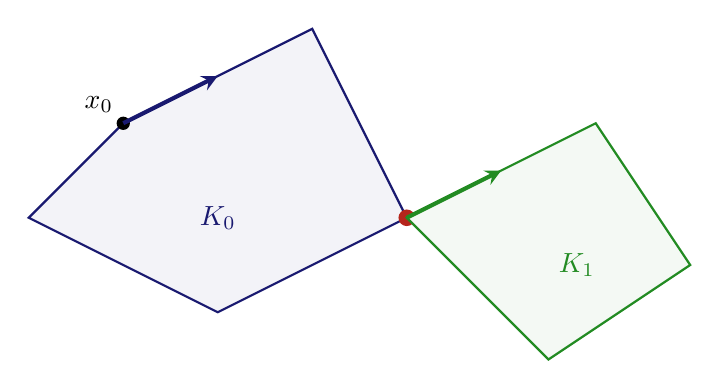
\begin{tikzpicture}[scale=1.2, >=stealth, thick]
  % \begin{ai-tikz-planner-invisible-content}
  % 1. Background: Kantenzug K_0 als lila Fünfeck.
  % 2. Midground: Kantenzug K_1 als grünes Viereck, das K_0 im Knoten x_n schneidet.
  % 3. Foreground: Pfeile, die den Durchlaufweg andeuten.
  % \end{ai-tikz-planner-invisible-content}
  
  % K_0 (lila)
  \draw[MidnightBlue, fill=MidnightBlue!5] (0,0) -- (2,1) -- (3,-1) -- (1,-2) -- (-1,-1) -- cycle;
  \node[MidnightBlue] at (1,-1) {$K_0$};
  \fill (0,0) circle (2pt) node[above left] {$x_0$};
  
  % Schnittknoten x_n
  \coordinate (Xn) at (3,-1);
  \fill[BrickRed] (Xn) circle (2.5pt) node[right=3pt] {$x_n$};
  
  % K_1 (grün)
  \draw[ForestGreen, fill=ForestGreen!5] (3,-1) -- (5,0) -- (6,-1.5) -- (4.5,-2.5) -- cycle;
  \node[ForestGreen] at (4.8,-1.5) {$K_1$};
  
  % Durchlaufpfeile
  \draw[->, MidnightBlue, line width=1.5pt] (0,0) -- (1,0.5);
  \draw[->, ForestGreen, line width=1.5pt] (3,-1) -- (4, -0.5);
\end{tikzpicture}
\end{center}

Da der Graph $G$ endlich ist, führt die wiederholte Anwendung dieses Verfahrens nach endlich vielen Schritten zu einem geschlossenen Kantenzug, der alle Kanten von $G$ enthält. Dies beweist, dass $G$ ein Euler-Graph ist.
\end{math-stroke}
\end{proof}

\begin{ai-global-state-checkpoint-invisible-content}
% timestamp: 00:18:00
% topic: Abschluss Satz von Euler, Einführung offene Euler-Linien
% board_state: prop:satz-von-euler, proof:euler-backward-complete
% next_goal: Formulierung des Korollars für offene Euler-Linien
% open_loops: none
\end{ai-global-state-checkpoint-invisible-content}

\subsection{Offene Euler-Linien}
% New subsection: Offene Euler-Linien

\begin{spoken-clean}[00:17:28 - 00:18:56]
Gut, soweit klar? Ich denke, die Idee des Beweises ist klar. Man kann das natürlich mehr oder weniger detailliert aufschreiben --- da gibt es verschiedene Möglichkeiten. Das hier ist eine Variante, vielleicht etwas kompakter, aber die Grundidee ist das Entscheidende.

Es gibt auch noch andere Versionen dieses Satzes, die wir hier nicht im Detail besprechen, die Sie aber im Skript nachlesen können. Bisher haben wir über geschlossene Euler-Linien gesprochen, aber man kann auch eine offene Euler-Linie definieren. Das ist ein Kantenzug, der zwar alle Kanten des Graphen $G$ enthält, aber nicht am selben Knoten beginnt, an dem er endet.

Auch hier lässt sich zeigen: Ein endlicher, ungerichteter Graph $G$ besitzt genau dann eine offene Euler-Linie, wenn er zusammenhängend ist und genau zwei Knoten mit ungeradem Grad existieren. In diesem Fall beginnen wir den Kantenzug an dem einen Knoten mit ungeradem Grad und beenden ihn an dem anderen.
\end{spoken-clean}

\begin{math-stroke}[Offene Euler-Linien]
\begin{definition}[Offene Euler-Linie]\label[definition]{def:offene-euler-linie}
Eine \newterm{offene Euler-Linie} in einem ungerichteten Graphen $G = (V, E)$ ist ein (nicht geschlossener) Kantenzug, der jede Kante von $G$ genau einmal enthält.
\end{definition}

\begin{corollary}[Existenz einer offenen Euler-Linie]\label[corollary]{cor:offene-euler-linie}
Ein endlicher, ungerichteter Graph $G$ besitzt genau dann eine offene Euler-Linie, wenn $G$ zusammenhängend ist (bis auf isolierte Knoten) und genau zwei Knoten $u, v \in V$ ungeraden Grad besitzen. In diesem Fall beginnt die offene Euler-Linie in $u$ und endet in $v$ (oder umgekehrt).
\end{corollary}
\end{math-stroke}

\begin{spoken-clean}[00:18:56 - 00:20:20]
Ähnliche Resultate gibt es auch für gerichtete Graphen --- das ist die Proposition 9.16 im Skript, die Sie dort gerne nachlesen können.
\end{spoken-clean}

\begin{math-stroke}[Weitere Versionen des Satzes]
\begin{remark}[Gerichtete Euler-Graphen]\label[remark]{rem:gerichtete-euler-graphen}
Für gerichtete Graphen gilt ein analoges Resultat (siehe Proposition 9.16 im Skript): Ein gerichteter, stark zusammenhängender Graph besitzt genau dann einen geschlossenen Euler-Zug, wenn für jeden Knoten der Eingangsgrad gleich dem Ausgangsgrad ist:
\[
\forall v \in V \colon d_{\text{in}}(v) = d_{\text{out}}(v)
\]
\end{remark}
\end{math-stroke}

\section{Das Dominoproblem}

\begin{spoken-clean}[00:20:20 - 00:22:30]
Kommen wir nun zu einer netten kleinen Anwendung dieses Satzes auf ein Problem aus dem Alltag: dem Dominoproblem. Ich weiß nicht, ob Sie heute noch oft Domino spielen, aber betrachten wir folgendes Szenario: Wir haben ein Dominospiel mit den Augenzahlen $0$ bis $16$ und den entsprechenden Dominosteinen.

Ein Dominostein sieht bekanntlich so aus: Er hat zwei Hälften mit jeweils einer Zahl, sagen wir $m$ und $n$, die beide zwischen $0$ und $16$ liegen. Für jedes ungeordnete Paar $\{m, n\}$ gibt es genau einen Stein --- es wird also nicht zwischen $\{m, n\}$ und $\{m, n\}$ unterschieden. Die Frage ist nun: Wie viele Steine hat ein solches Dominospiel insgesamt?
\end{spoken-clean}

\begin{math-stroke}[Mathematische Formulierung des Dominoproblems]
Wir betrachten ein Dominospiel mit den Augenzahlen $\{0, 1, \dots, 16\}$.
Ein Dominostein wird repräsentiert durch ein ungeordnetes Paar $\{m, n\}$ mit $m, n \in \{0, \dots, 16\}$. Für jedes Paar existiert genau ein Stein (inklusive der Doubletten $\{m, m\}$).
\end{math-stroke}

\begin{spoken-clean}[00:22:30 - 00:23:51]
Wie viele Möglichkeiten gibt es, zwei Zahlen aus $17$ auszuwählen? Dazu kommen noch die Doubletten, bei denen man zweimal dieselbe Zahl hat, also $0$-$0$, $1$-$1$ und so weiter. Das heißt, wir müssen noch $17$ weitere Steine dazuzählen.
\end{spoken-clean}

\begin{ai-global-state-checkpoint-invisible-content}
% timestamp: 00:24:00
% topic: Das Dominoproblem (Kombinatorik und Fragestellung)
% board_state: def:general-domino, eq:domino-count
% next_goal: Modellierung des Dominoproblems als Graph
% open_loops: none
\end{ai-global-state-checkpoint-invisible-content}

\begin{math-stroke}[Berechnung der Anzahl der Dominosteine]
Die Anzahl der Steine berechnet sich kombinatorisch aus den Paaren unterschiedlicher Zahlen plus den Doubletten (Steine mit zwei gleichen Zahlen):
\[
\text{Anzahl Steine} = \binom{17}{2} + 17 = \frac{17 \cdot 16}{2} + 17 = 136 + 17 = 153
\]
Es gibt somit insgesamt $153$ Dominosteine in diesem Spiel.
\end{math-stroke}

\begin{spoken-clean}[00:23:51 - 00:25:23]
Die spannende Frage beim Dominoproblem lautet nun: Können wir all diese Steine zu einer einzigen, unverzweigten, geschlossenen Kette aneinanderreihen?

Können wir die Steine also so anordnen, dass wir mit einem Stein $\{n_1, n_2\}$ beginnen, daran den Stein $\{n_2, n_3\}$ legen, und so weiter, bis wir am Ende wieder beim Ausgangswert $n_1$ ankommen?
\end{spoken-clean}

\begin{math-stroke}[Die Fragestellung]
\textbf{Frage:} Können wir alle $153$ Dominosteine so aneinanderreihen, dass sie eine einzige, geschlossene, unverzweigte Kette bilden?
\begin{center}
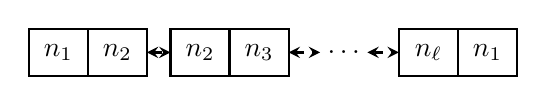
\begin{tikzpicture}[scale=1.0, >=stealth, thick]
  % \begin{ai-tikz-planner-invisible-content}
  % 1. Background: Eine Kette von Dominosteinen als Rechtecke.
  % 2. Midground: Zahlen auf den Steinen.
  % 3. Foreground: Verbindungslinien.
  % \end{ai-tikz-planner-invisible-content}
  \draw (0,0) rectangle (1.5,0.6);
  \draw (0.75,0) -- (0.75,0.6);
  \node at (0.375,0.3) {$n_1$};
  \node at (1.125,0.3) {$n_2$};
  
  \draw (1.8,0) rectangle (3.3,0.6);
  \draw (2.55,0) -- (2.55,0.6);
  \node at (2.175,0.3) {$n_2$};
  \node at (2.925,0.3) {$n_3$};
  
  \node at (4.0,0.3) {$\dots$};
  
  \draw (4.7,0) rectangle (6.2,0.6);
  \draw (5.45,0) -- (5.45,0.6);
  \node at (5.075,0.3) {$n_{\ell}$};
  \node at (5.825,0.3) {$n_1$};
  
  \draw[dashed, <->] (1.5,0.3) -- (1.8,0.3);
  \draw[dashed, <->] (3.3,0.3) -- (3.7,0.3);
  \draw[dashed, <->] (4.3,0.3) -- (4.7,0.3);
\end{tikzpicture}
\end{center}
\end{math-stroke}

\begin{spoken-clean}[00:25:23 - 00:26:25]
Was ist die Antwort? Überlegen Sie kurz, während ich die Tafel wische.

Es geht im Wesentlichen darum, einen passenden Graphen zu konstruieren und zu prüfen, ob dieser eine Euler-Linie besitzt oder nicht. Was meinen Sie, wie lautet die Antwort? Ja oder nein?

Wer von Ihnen tippt auf Ja? Okay. Wer denkt Nein? Und wer ist sich unsicher? \inlinemetanote{Der Dozent wischt die Wandtafel sauber, um Platz für den Beweis zu schaffen.}
\end{spoken-clean}

\begin{meta-note}[Tafelreinigung]
Der Dozent wischt die linke und mittlere Tafel vollständig, um die graphentheoretische Modellierung des Dominoproblems aufzuschreiben.
\end{meta-note}

\begin{spoken-clean}[00:26:25 - 00:28:18]
Die Antwort lautet tatsächlich: Ja! Das wäre eine hervorragende Clicker-Frage gewesen. Hat jemand eine Erklärung dafür?

Wir modellieren das Problem mit einem Graphen $G = (V, E)$. Als Knotenmenge $V$ wählen wir die Augenzahlen von $0$ bis $16$ --- wir haben also genau $17$ Knoten.

Eine Kante zwischen zwei Knoten existiert genau dann, wenn es den entsprechenden Dominostein gibt. Unsere Kanten repräsentieren also exakt die Dominosteine. Da jeder Dominostein zwei Zahlen miteinander verbindet, ist das eine sehr natürliche Modellierung. Die Kantenmenge $E$ besteht somit aus allen ungeordneten Paaren $\{a, b\}$ mit $a, b \in V$.
\end{spoken-clean}

\begin{math-stroke}[Graphentheoretische Modellierung des Dominoproblems]
\textbf{Antwort:} \textbf{JA}, eine solche Kette existiert immer.

\textbf{Beweis (Modellierung als Graph):}
Wir konstruieren einen Graphen $G = (V, E)$ wie folgt:
\begin{itemize}
    \item \textbf{Knotenmenge $V$:} Die Augenzahlen von $0$ bis $16$:
    \[
    V := \{0, 1, \dots, 16\} \implies |V| = 17.
    \]
    \item \textbf{Kantenmenge $E$:} Die Kanten entsprechen exakt den Dominosteinen. Da es für jedes Paar $\{a, b\}$ (inklusive der Doppelsteine $\{a, a\}$) genau einen Stein gibt, definieren wir:
    \[
    E := \bigl\{ \{a, b\} \;\big|\; a, b \in V \bigr\}.
    \]
\end{itemize}
\end{math-stroke}

\begin{spoken-clean}[00:28:18 - 00:29:55]
Hierbei sehen wir eine schöne Symmetrie. Zur Erinnerung: Ein Graph heißt regulär vom Grad $d$, wenn jeder Knoten den Grad $d$ besitzt.

Dieser Graph ist regulär vom Grad --- was meinen Sie? Genau, vom Grad $18$. Wenn wir einen beliebigen Knoten betrachten, können wir ihn mit jedem der anderen $16$ Knoten verbinden, was uns $16$ Kanten liefert.

Zusätzlich gibt es an jedem Knoten noch eine Schlinge zu sich selbst (für die Doubletten). Eine solche Schlinge erhöht den Knotengrad um $2$ --- das ist wie beim Händeschütteln mit sich selbst. Insgesamt ergibt das also $16 + 2 = 18$.
\end{spoken-clean}

\begin{spoken-clean}[00:29:55 - 00:31:34]
Im Prinzip haben wir hier den vollständigen Graphen $K_{17}$ --- das ist der einfache Graph vom Grad $16$, bei dem wir $17$ Knoten haben und jeden mit jedem anderen verbinden. An jeden dieser Knoten fügen wir nun noch eine Schlinge an, wir haben also zusätzlich $17$ Schlingen.

Da der Graph regulär vom Grad $18$ ist, hat jeder Knoten einen geraden Grad. Nach unserem Satz existiert somit eine geschlossene Euler-Linie.

Das ist eine sehr schöne Anwendung der Euler-Graphen auf ein konkretes Alltagsproblem. Wenn man ein anderes Dominospiel betrachten würde --- beispielsweise mit Augenzahlen nur bis $15$ ---, dann würde es nicht funktionieren. In diesem Fall hätten wir einen regulären Graphen vom Grad $17$, und da dieser ungerade ist, gäbe es keine Lösung.
\end{spoken-clean}

\begin{math-stroke}[Analyse des Graphen und Gradberechnung]
\begin{ai-global-state-checkpoint-invisible-content}
% timestamp: 00:31:00
% topic: Dominoproblem als Euler-Graph gelöst
% board_state: def:general-cartesian-product, prop:satz-von-euler
% next_goal: Abschluss des Beweises und Ausblick auf De-Bruijn-Folgen
% open_loops: none
\end{ai-global-state-checkpoint-invisible-content}

Der konstruierte Graph $G$ ist ein ungerichteter Graph mit Mehrfachkanten und Schleifen (Schlingen). Wir bestimmen den Grad eines beliebigen Knotens $v \in V$:
\begin{itemize}
    \item Es gibt genau $16$ Kanten zu allen anderen $16$ Knoten $u \neq v$ (entspricht den Steinen $\{v, u\}$).
    \item Es gibt genau $1$ Schlinge am Knoten $v$ (entspricht dem Doublettenstein $\{v, v\}$). Eine Schlinge erhöht den Grad des Knotens um genau $2$.
\end{itemize}
Daraus ergibt sich für jeden Knoten $v \in V$:
\[
\deg(v) = 16 + 2 = 18.
\]
Der Graph $G$ ist somit ein regulärer Graph vom Grad $18$. Wir können ihn darstellen als den vollständigen Graphen $K_{17}$ erweitert um eine Schlinge an jedem der $17$ Knoten:
\[
G = K_{17} \text{ mit } 17 \text{ Schlingen.}
\]

\textbf{Schlussfolgerung:}
\begin{enumerate}[label=\textbf{(\arabic*)}]
    \item Da $G$ zusammenhängend ist und jeder Knoten einen geraden Grad besitzt ($\deg(v) = 18 \equiv 0 \pmod 2$), existiert nach dem Satz von Euler (\cref{prop:satz-von-euler}) eine geschlossene Euler-Linie.
    \item Diese Euler-Linie entspricht einer geschlossenen, unverzweigten Kette, die jeden der $153$ Dominosteine genau einmal verwendet.
\end{enumerate}
\end{math-stroke}

\begin{didactic-insight}[Verallgemeinerung des Dominoproblems]
Die Lösbarkeit des Dominoproblems hängt entscheidend von der Parität der maximalen Augenzahl ab. 
\begin{itemize}
    \item Bei einer maximalen Augenzahl $N$ ist der Grad jedes Knotens im entsprechenden Graphen gleich $N + 2$.
    \item Ist $N$ gerade (wie im klassischen Spiel mit $N=6$ oder hier mit $N=16$), so ist der Grad $N+2$ ebenfalls gerade. Eine geschlossene Kette existiert somit immer!
    \item Ist $N$ jedoch ungerade (z.B. bei einem Spiel mit Augenzahlen $0$ bis $15$), so ist der Grad $N+2$ ungerade. In diesem Fall besitzt der Graph keine Euler-Linie, und eine vollständige geschlossene Kette ist mathematisch unmöglich!
\end{itemize}
\end{didactic-insight}

% --- TEIL 2 ---

\section{Hamilton-Kreise und Hamilton-Graphen}

\begin{spoken-clean}[00:31:34 - 00:32:29]
Soweit klar? Gibt es noch Fragen dazu? Gut. 

Dann gehen wir weiter zu einem anderen Konzept. Bisher haben wir Kantenzüge betrachtet, die jede Kante genau einmal durchlaufen. Nun können wir uns fragen: Was ist mit einem Kantenzug, der nicht zwingend alle Kanten, dafür aber alle Knoten genau einmal besucht? Wir suchen also nach einem Kreis --- das heißt einem geschlossenen Kantenzug, der jeden Knoten genau einmal enthält. Das führt uns zur folgenden Definition:
\end{spoken-clean}

\begin{math-stroke}
\begin{definition}[Hamilton-Kreis und Hamilton-Graph]\label[definition]{def:hamilton-kreis}
Sei $G = (V, E)$ ein ungerichteter, endlicher Graph.
\begin{itemize}
    \item Ein \newterm{Hamilton-Kreis} ist ein Kreis in $G$, der alle Knoten von $G$ enthält.
    \item Ein Graph $G$ heißt \newterm{Hamilton-Graph}, falls $G$ einen Hamilton-Kreis besitzt.
    \item Ein \newterm{Hamilton-Weg} ist ein einfacher Weg in $G$, der alle Knoten von $G$ enthält, aber nicht geschlossen sein muss.
\end{itemize}
\end{definition}
\end{math-stroke}

\begin{spoken-clean}[00:32:29 - 00:34:16]
Wir nennen einen Graphen $G$ einen Hamilton"=Graphen, falls er einen Hamilton"=Kreis besitzt.

Eine wichtige Bemerkung dazu: Im Gegensatz zu Euler"=Graphen gibt es für Hamilton"=Graphen leider kein einfaches, universelles Kriterium. Bei Euler"=Graphen müssen wir lediglich prüfen, ob alle Knotengrade gerade sind, und wissen sofort Bescheid.

Für Hamilton"=Graphen ist das Problem im Allgemeinen mathematisch sehr schwierig. Bei großen Graphen ist es extrem aufwendig zu entscheiden, ob ein solcher Kreis existiert. Es gibt jedoch einige klassische Beispiele, bei denen die Existenz leicht zu sehen ist. Das einfachste Beispiel ist der vollständige Graph $K_n$ für $n \ge 3$.
\end{spoken-clean}

\begin{ai-global-state-checkpoint-invisible-content}
% timestamp: 00:33:45
% topic: Einführung Hamilton-Kreise und Hamilton-Graphen
% board_state: def:hamilton-kreis
% next_goal: Beispiele für Hamilton-Graphen (K_n, Platonische Körper)
% open_loops: none
\end{ai-global-state-checkpoint-invisible-content}

\begin{math-stroke}[Der vollständige Graph \texorpdfstring{$K_n$}{K\_n}]
\begin{example}[Vollständige Graphen]\label[example]{ex:vollstaendige-graphen-hamilton}
Der vollständige Graph $K_n$ ist für alle $n \ge 3$ ein Hamilton-Graph.
\end{example}
\end{math-stroke}

\begin{spoken-clean}[00:34:16 - 00:35:22]
Das sieht man ganz leicht: Wir starten bei einem beliebigen Knoten $v_1$ und gehen zu einem Nachbarn $v_2$. Da im vollständigen Graphen jeder Knoten mit jedem anderen verbunden ist, können wir von $v_2$ aus jeden beliebigen unbesuchten Knoten wählen.

Wir können also von $v_2$ zu $v_3$ gehen, und so weiter, bis wir schließlich beim letzten Knoten $v_n$ ankommen. Da auch $v_n$ mit $v_1$ verbunden ist, können wir den Kreis schließen. Für den vollständigen Graphen $K_n$ ist die Sache also sehr einfach.
\end{spoken-clean}

\begin{math-stroke}[Visualisierung des Hamilton-Kreises in \texorpdfstring{$K_4$}{K\_4}]
\begin{center}
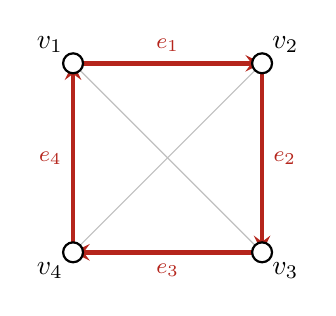
\begin{tikzpicture}[scale=1.2, thick, >=stealth]
  % \begin{ai-tikz-planner-invisible-content}
  % 1. Background: Vollständiger Graph K_4 mit dünnen grauen Kanten.
  % 2. Foreground: Der Hamilton-Kreis (v1 -> v2 -> v3 -> v4 -> v1) in dicker roter Linie.
  % 3. Nodes: Die vier Knoten v1, v2, v3, v4.
  % \end{ai-tikz-planner-invisible-content}
  
  % Coordinates
  \coordinate (V1) at (0,2);
  \coordinate (V2) at (2,2);
  \coordinate (V3) at (2,0);
  \coordinate (V4) at (0,0);
  
  % Background edges (non-cycle edges of K_4)
  \draw[gray!50, thin] (V1) -- (V3);
  \draw[gray!50, thin] (V2) -- (V4);
  
  % Hamilton Cycle (BrickRed, ultra thick)
  \draw[BrickRed, ultra thick, ->] (V1) -- (V2) node[midway, above] {\footnotesize $e_1$};
  \draw[BrickRed, ultra thick, ->] (V2) -- (V3) node[midway, right] {\footnotesize $e_2$};
  \draw[BrickRed, ultra thick, ->] (V3) -- (V4) node[midway, below] {\footnotesize $e_3$};
  \draw[BrickRed, ultra thick, ->] (V4) -- (V1) node[midway, left]  {\footnotesize $e_4$};
  
  % Nodes
  \filldraw[fill=white, draw=black] (V1) circle (3pt) node[above left] {$v_1$};
  \filldraw[fill=white, draw=black] (V2) circle (3pt) node[above right] {$v_2$};
  \filldraw[fill=white, draw=black] (V3) circle (3pt) node[below right] {$v_3$};
  \filldraw[fill=white, draw=black] (V4) circle (3pt) node[below left] {$v_4$};
\end{tikzpicture}
\end{center}
\end{math-stroke}

\subsection{Beispiele und platonische Körper}

\begin{spoken-clean}[00:35:22 - 00:36:46]
Ein weiteres, optisch sehr schönes Beispiel können wir über den Projektor betrachten. Ich zeige Ihnen dazu eine Abbildung. \inlinemetanote{schaltet den Projektor ein und zeigt eine Folie mit den platonischen Körpern}

Sie kennen sicherlich die platonischen Körper --- die fünf regulären Polyeder, bei denen alle Seitenflächen zueinander kongruente regelmäßige Vielecke sind. Es gibt genau fünf davon: Tetraeder, Würfel, Oktaeder, Dodekaeder und Ikosaeder. Das haben Sie bestimmt schon einmal in der Schule gesehen.

Wir können nun die Kantengraphen dieser Körper betrachten. Das bedeutet: Die Knoten des Graphen entsprechen den Ecken des Polyeders, und die Kanten des Graphen entsprechen den geometrischen Kanten. Jedem dieser platonischen Körper können wir so einen Graphen zuordnen. Auf der Folie sehen wir diese fünf Graphen mit ihren Knoten und Kanten.
\end{spoken-clean}

\begin{spoken-clean}[00:36:46 - 00:38:07]
Diese Graphen sind alle Hamilton-Graphen. Wir sehen hier die rot markierten Hamilton-Kreise.

Beim Tetraeder sehen wir im Kantengraphen direkt einen Kreis, der alle vier Knoten enthält. Auch beim Würfel können wir den Kantengraphen so zeichnen, dass sich ein klarer Hamilton-Kreis ergibt. Beim Oktaeder ist es genauso, wenn man den Graphen flach in die Ebene projiziert.

Dodekaeder und Ikosaeder sind etwas komplizierter. Man kann sich anschaulich vorstellen, dass man eine der Begrenzungsflächen ganz groß zieht und den Rest des Körpers flach hineindrückt --- so lassen sich diese Graphen übersichtlich als ebene Graphen darstellen. Und wie man auf den Abbildungen sieht, besitzen sie alle einen Hamilton-Kreis.
\end{spoken-clean}

\begin{math-stroke}[Kantengraphen der platonischen Körper]
\begin{example}[Platonische Körper]\label[example]{ex:platonische-koerper}
Die Kantengraphen der fünf platonischen Körper (Tetraeder, Würfel, Oktaeder, Dodekaeder, Ikosaeder) sind alle Hamilton-Graphen.
\end{example}

\begin{center}
\begin{tikzpicture}[scale=1.0, thick, >=stealth]
  % \begin{ai-tikz-planner-invisible-content}
  % 1. Background: Drei repräsentative platonische Kantengraphen (Tetraeder, Würfel, Oktaeder).
  % 2. Foreground: Hamilton-Kreise in BrickRed hervorgehoben.
  % \end{ai-tikz-planner-invisible-content}

  % --- TETRAEDER ---
  \begin{scope}[shift={(0,0)}]
    \coordinate (A) at (0,1.8);
    \coordinate (B) at (-1.5,-0.6);
    \coordinate (C) at (1.5,-0.6);
    \coordinate (D) at (0,0.2);
    
    % Non-cycle edges
    \draw[gray!40, thin] (A) -- (D);
    \draw[gray!40, thin] (B) -- (C);
    
    % Hamilton Cycle
    \draw[BrickRed, ultra thick] (A) -- (B) -- (D) -- (C) -- cycle;
    
    % Nodes
    \foreach \p in {A,B,C,D} \filldraw[fill=white, draw=black] (\p) circle (2.5pt);
    \node[below=0.8cm of B, xshift=1.5cm] {\textbf{Tetraeder}};
  \end{scope}

  % --- WÜRFEL ---
  \begin{scope}[shift={(4.5,0)}]
    \coordinate (A1) at (-1.2,1.2);
    \coordinate (B1) at (1.2,1.2);
    \coordinate (C1) at (1.2,-1.2);
    \coordinate (D1) at (-1.2,-1.2);
    
    \coordinate (A2) at (-0.6,0.6);
    \coordinate (B2) at (0.6,0.6);
    \coordinate (C2) at (0.6,-0.6);
    \coordinate (D2) at (-0.6,-0.6);
    
    % Non-cycle edges
    \draw[gray!40, thin] (A1) -- (B1);
    \draw[gray!40, thin] (C1) -- (D1);
    \draw[gray!40, thin] (A2) -- (D2);
    \draw[gray!40, thin] (B2) -- (C2);
    
    % Hamilton Cycle
    \draw[BrickRed, ultra thick] (A1) -- (A2) -- (B2) -- (B1) -- (C1) -- (C2) -- (D2) -- (D1) -- cycle;
    
    % Nodes
    \foreach \p in {A1,B1,C1,D1,A2,B2,C2,D2} \filldraw[fill=white, draw=black] (\p) circle (2.5pt);
    \node[below=1.4cm of D1, xshift=1.2cm] {\textbf{Würfel}};
  \end{scope}

  % --- OKTAEDER ---
  \begin{scope}[shift={(9,0)}]
    \coordinate (U) at (0,1.5);
    \coordinate (D) at (0,-1.5);
    \coordinate (L) at (-1.5,0);
    \coordinate (R) at (1.5,0);
    \coordinate (I1) at (-0.5,-0.3);
    \coordinate (I2) at (0.5,0.3);
    
    % Non-cycle edges
    \draw[gray!40, thin] (U) -- (D);
    \draw[gray!40, thin] (L) -- (R);
    
    % Hamilton Cycle
    \draw[BrickRed, ultra thick] (U) -- (L) -- (I1) -- (D) -- (R) -- (I2) -- cycle;
    
    % Nodes
    \foreach \p in {U,D,L,R,I1,I2} \filldraw[fill=white, draw=black] (\p) circle (2.5pt);
    \node[below=1.7cm of L, xshift=1.5cm] {\textbf{Oktaeder}};
  \end{scope}
\end{tikzpicture}
\end{center}
\end{math-stroke}

\subsection{Der \texorpdfstring{$k$}{k}-dimensionale Würfel und Gray-Codes}

\begin{spoken-clean}[00:38:07 - 00:40:08]
Ein weiteres interessantes Beispiel ist der Kantengraph eines Hyperwürfels beliebiger Dimension $k$. \inlinemetanote{schreibt an die Tafel}

Für $k=2$ erhalten wir einfach das Quadrat. Ein zweidimensionaler Würfel ist ein Quadrat, und dort können wir offensichtlich einmal im Kreis herumlaufen --- das ist ein Hamilton-Kreis.

Für $k=3$ --- den klassischen dreidimensionalen Würfel --- müssen wir auch nicht allzu lange überlegen. Ich zeichne den Weg einmal farbig ein: Wir können beispielsweise so laufen, dann nach oben, rüber, nach hinten, und über die verbleibenden Ecken wieder zurück nach vorne zum Startpunkt. Das ergibt einen geschlossenen Kreis, bei dem jeder Knoten exakt einmal besucht wird.
\end{spoken-clean}

\begin{math-stroke}[Der \texorpdfstring{$k$}{k}-dimensionale Würfel \texorpdfstring{$Q_k$}{Q\_k}]
\begin{definition}[$k$-dimensionaler Würfel]\label[definition]{def:k-dim-cube}
Der \newterm{$k$-dimensionaler Würfel} (oder Hyperwürfel) $Q_k$ ist der ungerichtete Graph, dessen Knotenmenge $V = \{0, 1\}^k$ aus allen binären Wörtern der Länge $k$ besteht. Zwei Knoten $a, b \in V$ sind genau dann durch eine Kante verbunden, wenn sie sich in genau einer Koordinate unterscheiden.
\end{definition}

% \begin{center}
% \begin{tikzpicture}[scale=1.4, thick, >=stealth]
%   % Coordinates Front Face
%   \coordinate (000) at (0, 0);
%   \coordinate (100) at (3.6, 0);
%   \coordinate (110) at (3.6, 3.6);
%   \coordinate (010) at (0, 3.6);
  
%   % Coordinates Back Face (offset for clean 3D perspective)
%   \coordinate (001) at (1.7, 1.5);
%   \coordinate (101) at (5.3, 1.5);
%   \coordinate (111) at (5.3, 5.1);
%   \coordinate (011) at (1.7, 5.1);
  
%   % 1. Background / Non-Hamilton Edges (Gray, dashed/subtle for depth)
%   \draw[gray!50, line width=1.3pt, dashed] (000) -- (010);
%   \draw[gray!50, line width=1.3pt, dashed] (100) -- (101);
%   \draw[gray!50, line width=1.3pt, dashed] (110) -- (111);
%   \draw[gray!50, line width=1.3pt, dashed] (001) -- (011);
  
%   % 2. Hamilton Cycle / Gray-Code Path (BrickRed, bold, with directional arrows)
%   % Back face part of cycle: 010 -> 011 -> 111 -> 101 -> 001 -> 000
%   \draw[->, BrickRed, line width=2.2pt] (010) -- (011);
%   \draw[->, BrickRed, line width=2.2pt] (011) -- (111);
%   \draw[->, BrickRed, line width=2.2pt] (111) -- (101);
%   \draw[->, BrickRed, line width=2.2pt] (101) -- (001);
%   \draw[->, BrickRed, line width=2.2pt] (001) -- (000);
  
%   % Front face part of cycle: 000 -> 100 -> 110 -> 010
%   \draw[->, BrickRed, line width=2.2pt] (000) -- (100);
%   \draw[->, BrickRed, line width=2.2pt] (100) -- (110);
%   \draw[->, BrickRed, line width=2.2pt] (110) -- (010);
  
%   % 3. Vertices (Styled as clean circles with shadows)
%   % Back vertices first (for proper layering)
%   \node[circle, draw=ThemeSecondary, fill=white, line width=1.2pt, inner sep=3pt, drop shadow] at (001) {};
%   \node[circle, draw=ThemeSecondary, fill=white, line width=1.2pt, inner sep=3pt, drop shadow] at (101) {};
%   \node[circle, draw=ThemeSecondary, fill=white, line width=1.2pt, inner sep=3pt, drop shadow] at (111) {};
%   \node[circle, draw=ThemeSecondary, fill=white, line width=1.2pt, inner sep=3pt, drop shadow] at (011) {};
  
%   % Front vertices
%   \node[circle, draw=ThemePrimary, fill=white, line width=1.4pt, inner sep=3.2pt, drop shadow] at (000) {};
%   \node[circle, draw=ThemePrimary, fill=white, line width=1.4pt, inner sep=3.2pt, drop shadow] at (100) {};
%   \node[circle, draw=ThemePrimary, fill=white, line width=1.4pt, inner sep=3.2pt, drop shadow] at (110) {};
%   \node[circle, draw=ThemePrimary, fill=white, line width=1.4pt, inner sep=3.2pt, drop shadow] at (010) {};
  
%   % 4. Labels with custom offsets and white backgrounds to prevent line overlap
%   \node[font=\sffamily\footnotesize\bfseries, text=ThemeSecondary, fill=white, inner xsep=2pt, inner ysep=1pt, rounded corners=2pt] at ($(001)+(-0.35,0.25)$) {$001$};
%   \node[font=\sffamily\footnotesize\bfseries, text=ThemeSecondary, fill=white, inner xsep=2pt, inner ysep=1pt, rounded corners=2pt] at ($(101)+(0.4,-0.2)$) {$101$};
%   \node[font=\sffamily\footnotesize\bfseries, text=ThemeSecondary, fill=white, inner xsep=2pt, inner ysep=1pt, rounded corners=2pt] at ($(111)+(0.4,0.25)$) {$111$};
%   \node[font=\sffamily\footnotesize\bfseries, text=ThemeSecondary, fill=white, inner xsep=2pt, inner ysep=1pt, rounded corners=2pt] at ($(011)+(-0.35,0.25)$) {$011$};
  
%   \node[font=\sffamily\footnotesize\bfseries, text=ThemePrimary, fill=white, inner xsep=2pt, inner ysep=1pt, rounded corners=2pt] at ($(000)+(-0.4,-0.3)$) {$000$};
%   \node[font=\sffamily\footnotesize\bfseries, text=ThemePrimary, fill=white, inner xsep=2pt, inner ysep=1pt, rounded corners=2pt] at ($(100)+(0.4,-0.3)$) {$100$};
%   \node[font=\sffamily\footnotesize\bfseries, text=ThemePrimary, fill=white, inner xsep=2pt, inner ysep=1pt, rounded corners=2pt] at ($(110)+(0.4,0.3)$) {$110$};
%   \node[font=\sffamily\footnotesize\bfseries, text=ThemePrimary, fill=white, inner xsep=2pt, inner ysep=1pt, rounded corners=2pt] at ($(010)+(-0.4,0.3)$) {$010$};
  
%   % 5. Explanatory Legend / Caption badge below
%   \node[draw=ThemePrimary!60, fill=ThemeBgLight, rounded corners=4pt, inner xsep=10pt, inner ysep=6pt, font=\sffamily\small, drop shadow] at (2.65, -1.2) {
%     \begin{tabular}{c}
%       \textbf{\textcolor{BrickRed}{Roter Pfeilpfad:}} Hamilton-Kreis im $Q_3$ \\
%       \footnotesize Zyklischer Gray-Code: $000 \to 100 \to 110 \to 010 \to 011 \to 111 \to 101 \to 001 \to 000$
%     \end{tabular}
%   };
% \end{tikzpicture}
% \end{center}

% \begin{center}
% \begin{tikzpicture}[scale=1.4, thick, >=stealth]
%   \begin{ai-tikz-planner-invisible-content}
%   % 1. Background: 3D-Würfel Q_3 in sauberer Kabinett-Projektion mit gestrichelten grauen Kanten (gray!50, dashed) für Tiefenwirkung.
%   % 2. Foreground: Ein mathematisch korrekter Hamilton-Kreis (Gray-Code: 000 -> 100 -> 110 -> 010 -> 011 -> 111 -> 101 -> 001 -> 000) in dicker roter Linie (BrickRed, line width=2.2pt) mit gerichteten Pfeilen.
%   % 3. Styling: Knoten als weiße Kreise mit drop shadow, farbliche Kennzeichnung (ThemePrimary vs. ThemeSecondary) zur didaktischen Trennung der vorderen und hinteren Würfelebene.
%   % 4. Labels: Eigens positionierte Textknoten mit weißer Füllung gegen Kanten-Kollisionen. Explikative Tabellen-Legende unter der Grafik.
%   \end{ai-tikz-planner-invisible-content}

%   % Coordinates Front Face
%   \coordinate (000) at (0, 0);
%   \coordinate (100) at (3.6, 0);
%   \coordinate (110) at (3.6, 3.6);
%   \coordinate (010) at (0, 3.6);
  
%   % Coordinates Back Face (offset for clean 3D perspective)
%   \coordinate (001) at (1.7, 1.5);
%   \coordinate (101) at (5.3, 1.5);
%   \coordinate (111) at (5.3, 5.1);
%   \coordinate (011) at (1.7, 5.1);
  
%   % 1. Background / Non-Hamilton Edges (Gray, dashed/subtle for depth)
%   \draw[gray!50, line width=1.3pt, dashed] (000) -- (010);
%   \draw[gray!50, line width=1.3pt, dashed] (100) -- (101);
%   \draw[gray!50, line width=1.3pt, dashed] (110) -- (111);
%   \draw[gray!50, line width=1.3pt, dashed] (001) -- (011);
  
%   % 2. Hamilton Cycle / Gray-Code Path (BrickRed, bold, with directional arrows)
%   % Back face part of cycle: 010 -> 011 -> 111 -> 101 -> 001 -> 000
%   \draw[->, BrickRed, line width=2.2pt] (010) -- (011);
%   \draw[->, BrickRed, line width=2.2pt] (011) -- (111);
%   \draw[->, BrickRed, line width=2.2pt] (111) -- (101);
%   \draw[->, BrickRed, line width=2.2pt] (101) -- (001);
%   \draw[->, BrickRed, line width=2.2pt] (001) -- (000);
  
%   % Front face part of cycle: 000 -> 100 -> 110 -> 010
%   \draw[->, BrickRed, line width=2.2pt] (000) -- (100);
%   \draw[->, BrickRed, line width=2.2pt] (100) -- (110);
%   \draw[->, BrickRed, line width=2.2pt] (110) -- (010);
  
%   % 3. Vertices (Styled as clean circles with shadows)
%   % Back vertices first (for proper layering)
%   \node[circle, draw=ThemeSecondary, fill=white, line width=1.2pt, inner sep=3pt, drop shadow] at (001) {};
%   \node[circle, draw=ThemeSecondary, fill=white, line width=1.2pt, inner sep=3pt, drop shadow] at (101) {};
%   \node[circle, draw=ThemeSecondary, fill=white, line width=1.2pt, inner sep=3pt, drop shadow] at (111) {};
%   \node[circle, draw=ThemeSecondary, fill=white, line width=1.2pt, inner sep=3pt, drop shadow] at (011) {};
  
%   % Front vertices
%   \node[circle, draw=ThemePrimary, fill=white, line width=1.4pt, inner sep=3.2pt, drop shadow] at (000) {};
%   \node[circle, draw=ThemePrimary, fill=white, line width=1.4pt, inner sep=3.2pt, drop shadow] at (100) {};
%   \node[circle, draw=ThemePrimary, fill=white, line width=1.4pt, inner sep=3.2pt, drop shadow] at (110) {};
%   \node[circle, draw=ThemePrimary, fill=white, line width=1.4pt, inner sep=3.2pt, drop shadow] at (010) {};
  
%   % 4. Labels with custom offsets and white backgrounds to prevent line overlap
%   \node[font=\sffamily\footnotesize\bfseries, text=ThemeSecondary, fill=white, inner xsep=2pt, inner ysep=1pt, rounded corners=2pt] at ($(001)+(-0.35,0.25)$) {$001$};
%   \node[font=\sffamily\footnotesize\bfseries, text=ThemeSecondary, fill=white, inner xsep=2pt, inner ysep=1pt, rounded corners=2pt] at ($(101)+(0.4,-0.2)$) {$101$};
%   \node[font=\sffamily\footnotesize\bfseries, text=ThemeSecondary, fill=white, inner xsep=2pt, inner ysep=1pt, rounded corners=2pt] at ($(111)+(0.4,0.25)$) {$111$};
%   \node[font=\sffamily\footnotesize\bfseries, text=ThemeSecondary, fill=white, inner xsep=2pt, inner ysep=1pt, rounded corners=2pt] at ($(011)+(-0.35,0.25)$) {$011$};
  
%   \node[font=\sffamily\footnotesize\bfseries, text=ThemePrimary, fill=white, inner xsep=2pt, inner ysep=1pt, rounded corners=2pt] at ($(000)+(-0.4,-0.3)$) {$000$};
%   \node[font=\sffamily\footnotesize\bfseries, text=ThemePrimary, fill=white, inner xsep=2pt, inner ysep=1pt, rounded corners=2pt] at ($(100)+(0.4,-0.3)$) {$100$};
%   \node[font=\sffamily\footnotesize\bfseries, text=ThemePrimary, fill=white, inner xsep=2pt, inner ysep=1pt, rounded corners=2pt] at ($(110)+(0.4,0.3)$) {$110$};
%   \node[font=\sffamily\footnotesize\bfseries, text=ThemePrimary, fill=white, inner xsep=2pt, inner ysep=1pt, rounded corners=2pt] at ($(010)+(-0.4,0.3)$) {$010$};
  
%   % 5. Explanatory Legend / Caption badge below
%   \node[draw=ThemePrimary!60, fill=ThemeBgLight, rounded corners=4pt, inner xsep=10pt, inner ysep=6pt, font=\sffamily\small, drop shadow] at (2.65, -1.2) {
%     \begin{tabular}{c}
%       \textbf{\textcolor{BrickRed}{Roter Pfeilpfad:}} Hamilton-Kreis im $Q_3$ \\
%       \footnotesize Zyklischer Gray-Code: $000 \to 100 \to 110 \to 010 \to 011 \to 111 \to 101 \to 001 \to 000$
%     \end{tabular}
%   };
% \end{tikzpicture}
% \end{center}

\begin{center}
\begin{tikzpicture}[scale=1.4, thick, >=stealth]
  \begin{ai-tikz-planner-invisible-content}
  % 1. Background: 3D-Würfel Q_3 in sauberer Kabinett-Projektion mit gestrichelten grauen Kanten (gray!50, dashed) für Tiefenwirkung.
  % 2. Foreground Layering: Knoten werden zuerst gezeichnet, und der Hamilton-Kreis (Gray-Code: 000 -> 100 -> 110 -> 010 -> 011 -> 111 -> 101 -> 001 -> 000) wird danach als gerichtete Pfeile (BrickRed, line width=2.2pt) über die Knoten hinweg gezeichnet, wobei auf die benannten Knoten (n000 bis n111) referenziert wird. Dadurch liegen die Pfeile im Vordergrund und enden sauber an den Knotengrenzen.
  % 3. Styling: Knoten als weiße Kreise mit drop shadow, farbliche Kennzeichnung (ThemePrimary vs. ThemeSecondary) zur didaktischen Trennung der vorderen und hinteren Würfelebene.
  % 4. Labels: Eigens positionierte Textknoten mit weißer Füllung gegen Kanten-Kollisionen. Explikative Tabellen-Legende unter der Grafik.
  \end{ai-tikz-planner-invisible-content}

  % Coordinates Front Face
  \coordinate (000) at (0, 0);
  \coordinate (100) at (3.6, 0);
  \coordinate (110) at (3.6, 3.6);
  \coordinate (010) at (0, 3.6);
  
  % Coordinates Back Face (offset for clean 3D perspective)
  \coordinate (001) at (1.7, 1.5);
  \coordinate (101) at (5.3, 1.5);
  \coordinate (111) at (5.3, 5.1);
  \coordinate (011) at (1.7, 5.1);
  
  % 1. Background / Non-Hamilton Edges (Gray, dashed/subtle for depth)
  \draw[gray!50, line width=1.3pt, dashed] (000) -- (010);
  \draw[gray!50, line width=1.3pt, dashed] (100) -- (101);
  \draw[gray!50, line width=1.3pt, dashed] (110) -- (111);
  \draw[gray!50, line width=1.3pt, dashed] (001) -- (011);
  
  % 2. Vertices (Styled as clean circles with shadows) - Drawn BEFORE the Hamilton cycle path
  % Back vertices first (for proper layering)
  \node (n001) [circle, draw=ThemeSecondary, fill=white, line width=1.2pt, inner sep=3pt, drop shadow] at (001) {};
  \node (n101) [circle, draw=ThemeSecondary, fill=white, line width=1.2pt, inner sep=3pt, drop shadow] at (101) {};
  \node (n111) [circle, draw=ThemeSecondary, fill=white, line width=1.2pt, inner sep=3pt, drop shadow] at (111) {};
  \node (n011) [circle, draw=ThemeSecondary, fill=white, line width=1.2pt, inner sep=3pt, drop shadow] at (011) {};
  
  % Front vertices
  \node (n000) [circle, draw=ThemePrimary, fill=white, line width=1.4pt, inner sep=3.2pt, drop shadow] at (000) {};
  \node (n100) [circle, draw=ThemePrimary, fill=white, line width=1.4pt, inner sep=3.2pt, drop shadow] at (100) {};
  \node (n110) [circle, draw=ThemePrimary, fill=white, line width=1.4pt, inner sep=3.2pt, drop shadow] at (110) {};
  \node (n010) [circle, draw=ThemePrimary, fill=white, line width=1.4pt, inner sep=3.2pt, drop shadow] at (010) {};
  
  % 3. Hamilton Cycle / Gray-Code Path in Foreground (BrickRed, bold, with directional arrows)
  % Back face part of cycle: 010 -> 011 -> 111 -> 101 -> 001 -> 000
  \draw[->, BrickRed, line width=2.2pt] (n010) -- (n011);
  \draw[->, BrickRed, line width=2.2pt] (n011) -- (n111);
  \draw[->, BrickRed, line width=2.2pt] (n111) -- (n101);
  \draw[->, BrickRed, line width=2.2pt] (n101) -- (n001);
  \draw[->, BrickRed, line width=2.2pt] (n001) -- (n000);
  
  % Front face part of cycle: 000 -> 100 -> 110 -> 010
  \draw[->, BrickRed, line width=2.2pt] (n000) -- (n100);
  \draw[->, BrickRed, line width=2.2pt] (n100) -- (n110);
  \draw[->, BrickRed, line width=2.2pt] (n110) -- (n010);
  
  % 4. Labels with custom offsets and white backgrounds to prevent line overlap
  \node[font=\sffamily\footnotesize\bfseries, text=ThemeSecondary, fill=white, inner xsep=2pt, inner ysep=1pt, rounded corners=2pt] at ($(001)+(-0.35,0.25)$) {$001$};
  \node[font=\sffamily\footnotesize\bfseries, text=ThemeSecondary, fill=white, inner xsep=2pt, inner ysep=1pt, rounded corners=2pt] at ($(101)+(0.4,-0.2)$) {$101$};
  \node[font=\sffamily\footnotesize\bfseries, text=ThemeSecondary, fill=white, inner xsep=2pt, inner ysep=1pt, rounded corners=2pt] at ($(111)+(0.4,0.25)$) {$111$};
  \node[font=\sffamily\footnotesize\bfseries, text=ThemeSecondary, fill=white, inner xsep=2pt, inner ysep=1pt, rounded corners=2pt] at ($(011)+(-0.35,0.25)$) {$011$};
  
  \node[font=\sffamily\footnotesize\bfseries, text=ThemePrimary, fill=white, inner xsep=2pt, inner ysep=1pt, rounded corners=2pt] at ($(000)+(-0.4,-0.3)$) {$000$};
  \node[font=\sffamily\footnotesize\bfseries, text=ThemePrimary, fill=white, inner xsep=2pt, inner ysep=1pt, rounded corners=2pt] at ($(100)+(0.4,-0.3)$) {$100$};
  \node[font=\sffamily\footnotesize\bfseries, text=ThemePrimary, fill=white, inner xsep=2pt, inner ysep=1pt, rounded corners=2pt] at ($(110)+(0.4,0.3)$) {$110$};
  \node[font=\sffamily\footnotesize\bfseries, text=ThemePrimary, fill=white, inner xsep=2pt, inner ysep=1pt, rounded corners=2pt] at ($(010)+(-0.4,0.3)$) {$010$};
  
  % 5. Explanatory Legend / Caption badge below
  \node[draw=ThemePrimary!60, fill=ThemeBgLight, rounded corners=4pt, inner xsep=10pt, inner ysep=6pt, font=\sffamily\small, drop shadow] at (2.65, -1.2) {
    \begin{tabular}{c}
      \textbf{\textcolor{BrickRed}{Roter Pfeilpfad:}} Hamilton-Kreis im $Q_3$ \\
      \footnotesize Zyklischer Gray-Code: $000 \to 100 \to 110 \to 010 \to 011 \to 111 \to 101 \to 001 \to 000$
    \end{tabular}
  };
\end{tikzpicture}
\end{center}
\end{math-stroke}

\begin{spoken-clean}[00:41:24 - 00:42:44]
Für ein beliebiges $k$ können wir uns den $k$-dimensionalen Würfel wie folgt vorstellen: Wir betrachten im $\mathbb{R}^k$ alle Punkte, deren Koordinaten ausschließlich aus Nullen und Einsen bestehen --- das sind unsere Knoten. Zwei Knoten sind genau dann durch eine Kante verbunden, wenn sie sich in genau einer Koordinate unterscheiden.

Das bedeutet, wir identifizieren die $2^k$ Ecken des $k$-dimensionalen Würfels mit den binären Wörtern der Länge $k$.
\end{spoken-clean}

\begin{spoken-clean}[00:42:44 - 00:43:45]
Wir identifizieren die $2^k$ Ecken des $k$-dimensionalen Würfels mit binären Wörtern der Länge $k$, also mit den Elementen aus $\{0, 1\}^k$. Zwei Wörter $a, b \in \{0, 1\}^k$ sind genau dann durch eine Kante verbunden, wenn sie sich in exakt einer Stelle unterscheiden.
\end{spoken-clean}

\begin{spoken-clean}[00:43:45 - 00:46:50]
Wir wollen zeigen, dass eine solche zyklische Folge existiert, bei der sich von Schritt zu Schritt immer nur ein einziges Bit ändert und wir am Ende wieder beim Startwort ankommen. Eine solche Folge nennt man einen Gray-Code.

Der Name stammt historisch aus der Codierungstheorie, in der man untersucht, wie man Codewörter so wählt, dass man Informationen möglichst fehlerresistent übertragen kann --- Stichwort fehlerkorrigierende Codes. Aber das ist für uns an dieser Stelle nicht weiter wichtig.

Für uns ist der mathematische Beweis entscheidend, dass eine solche Folge für jede Dimension $k$ existiert. Der Beweis ist erfreulich einfach und erfolgt per vollständiger Induktion nach $k$.
\end{spoken-clean}

\begin{math-stroke}[Existenz von Gray-Codes]
\begin{proposition}[Existenz von Gray-Codes]\label[proposition]{prop:gray-code-existenz}
Für jedes $k \ge 1$ existiert eine zyklische Folge $(a_1, \dots, a_{2^k})$ aller $2^k$ verschiedenen binären Wörter der Länge $k$, sodass sich aufeinanderfolgende Wörter $a_{\ell}$ und $a_{\ell+1}$ (sowie das letzte Wort $a_{2^k}$ und das erste Wort $a_1$) in genau einer Stelle unterscheiden. Ein solcher Zyklus entspricht genau einem Hamilton-Kreis im Hyperwürfel $Q_k$.
\end{proposition}
\end{math-stroke}

\begin{proof}[Beweis der Existenz von Gray-Codes]
\begin{spoken-clean}[00:46:50 - 00:48:18]
Wir führen den Beweis per Induktion nach $k$. Der Induktionsanfang für $k=1$ ist trivial: Bei Wörtern der Länge $1$ nehmen wir einfach die Folge $(0, 1)$. Die beiden Wörter unterscheiden sich in genau einer Stelle, und der Rückweg von $1$ zu $0$ ebenfalls.

Für den Induktionsschritt von $k$ auf $k+1$ nehmen wir an, dass bereits ein zyklischer Gray-Code der Länge $2^k$ existiert, den wir als $(a_1, \dots, a_{2^k})$ schreiben.
\end{spoken-clean}

\begin{spoken-clean}[00:48:18 - 00:49:28]
Daraus konstruieren wir nun einen Gray-Code für die Dimension $k+1$. Das machen wir wie folgt: Zuerst stellen wir allen Wörtern unseres bekannten Codes eine $0$ voran, wir bilden also die Folge $(0a_1, 0a_2, \dots, 0a_{2^k})$.
\end{spoken-clean}

\begin{spoken-clean}[00:49:28 - 00:50:58]
Diese Wörter unterscheiden sich untereinander weiterhin jeweils nur in einer Stelle, da dies bereits für die $a_i$ galt. Als nächstes Element wählen wir $1a_{2^k}$. Dieses unterscheidet sich vom vorherigen Wort $0a_{2^k}$ ebenfalls nur in einer einzigen Stelle --- nämlich der neu hinzugefügten ersten Stelle.

Anschließend spiegeln wir die restliche Folge und stellen jeweils eine $1$ voran: Wir gehen also rückwärts von $1a_{2^k-1}$ bis $1a_1$.
\end{spoken-clean}

\begin{spoken-clean}[00:50:58 - 00:52:40]
Diese Wörter unterscheiden sich aufeinanderfolgend ebenfalls jeweils nur in einer Stelle. Am Ende schließt sich der Kreis vom letzten Wort $1a_1$ zurück zum ersten Wort $0a_1$ wiederum durch die Änderung von genau einer Stelle --- nämlich der ersten. Damit haben wir einen gültigen Gray-Code für $k+1$ konstruiert.
\end{spoken-clean}

\begin{math-stroke}
Wir führen den Beweis per vollständiger Induktion nach der Dimension $k$:
\begin{itemize}
    \item \textbf{Induktionsanfang ($k=1$):} Die Folge $(a_1, a_2) := (0, 1)$ ist ein zyklischer Gray-Code der Länge $2^1 = 2$, da sich $0$ und $1$ in genau einer Stelle unterscheiden.
    \item \textbf{Induktionsschritt ($k \to k+1$):} Sei $(a_1, a_2, \dots, a_{2^k})$ ein zyklischer Gray-Code der Länge $2^k$. Wir konstruieren eine neue Folge $(b_1, \dots, b_{2^{k+1}})$ der Länge $2^{k+1}$ durch Spiegelung und Voranstellen von $0$ bzw. $1$:
    \[
    b_i := \begin{cases}
    0a_i & \text{für } 1 \le i \le 2^k \\
    1a_{2^{k+1} - i + 1} & \text{für } 2^k + 1 \le i \le 2^{k+1}
    \end{cases}
    \]
    Wir verifizieren die Gray-Code-Eigenschaften für die Übergänge:
    \begin{enumerate}[label=\textbf{(\arabic*)}]
        \item \textbf{Innerhalb der ersten Hälfte ($1 \le i < 2^k$):} $b_i = 0a_i$ und $b_{i+1} = 0a_{i+1}$ unterscheiden sich nur in einer Stelle, da sich $a_i$ und $a_{i+1}$ nach Induktionsvoraussetzung nur in einer Stelle unterscheiden.
        \item \textbf{Am Übergangspunkt ($i = 2^k$):} $b_{2^k} = 0a_{2^k}$ und $b_{2^k+1} = 1a_{2^k}$ unterscheiden sich exakt nur in der ersten (vorangestellten) Stelle.
        \item \textbf{Innerhalb der zweiten Hälfte ($2^k + 1 \le i < 2^{k+1}$):} $b_i = 1a_{2^{k+1}-i+1}$ und $b_{i+1} = 1a_{2^{k+1}-i}$ unterscheiden sich analog zur ersten Hälfte nur in einer Stelle.
        \item \textbf{Am zyklischen Rücklauf ($i = 2^{k+1}$):} Das letzte Element $b_{2^{k+1}} = 1a_1$ und das erste Element $b_1 = 0a_1$ unterscheiden sich ebenfalls exakt nur in der ersten Stelle.
    \end{enumerate}
    Die konstruierte Folge ist somit ein wohldefinierter, zyklischer Gray-Code der Länge $2^{k+1}$.
\end{itemize}
\end{math-stroke}
\end{proof}

\begin{spoken-clean}[00:52:40 - 00:54:38]
Das ist ein weiteres schönes Beispiel für Hamilton-Graphen. Solche Hyperwürfel bekommen sehr schnell extrem viele Ecken und Kanten: Ein eindimensionaler Würfel hat $2$ Ecken, ein zweidimensionaler $4$, ein dreidimensionaler $8$, und der vierdimensionale Würfel besitzt bereits $16$ Ecken. Das ist geometrisch nicht mehr ganz so einfach zu visualisieren, aber es ist bereits ein recht großer Graph.

Auf der Folie sehen Sie ein Beispiel dafür, wie ein Hamilton-Kreis im vierdimensionalen Würfel aussieht. Hier sind alle $16$ Ecken dargestellt, und wir können einen möglichen Gray-Code ablaufen. Man sieht sehr schön, dass sich von Schritt zu Schritt immer nur genau eine einzige Stelle verändert.

Die rote Linie zeigt den Hamilton-Kreis im projizierten Kantengraphen des vierdimensionalen Würfels. Sie können gerne nachprüfen, dass dieser Weg tatsächlich jeden der $16$ Knoten genau einmal besucht und am Ende wieder geschlossen ist. Solche Hyperwürfel sind mathematisch sehr elegant und einfach zu definieren, aber anschaulich manchmal gar nicht so leicht zu greifen.
\end{spoken-clean}

\begin{meta-note}[Tafelreinigung]
Der Dozent wischt die Tafel gründlich, um Platz für das nächste Thema zu schaffen, während auf dem Projektor eine Folie des vierdimensionalen Hyperwürfels ($Q_4$, Tesseract) mit einem rot markierten Hamilton-Kreis zu sehen ist.
\end{meta-note}

% \begin{math-stroke}[Der vierdimensionale Hyperwürfel \texorpdfstring{$Q_4$}{Q\_4}]
% \begin{center}
% \begin{tikzpicture}[scale=1.5, thick, >=stealth]
%   % \begin{ai-tikz-planner-invisible-content}
%   % 1. Background: Projektion des Tesseracts (Q_4) mit dünnen grauen Linien.
%   % 2. Foreground: Ein Hamilton-Kreis (Gray-Code) in dicker roter Linie (BrickRed).
%   % \end{ai-tikz-planner-invisible-content}
  
%   % Inner Cube Coordinates
%   \coordinate (0000) at (-0.5,-0.5,-0.5);
%   \coordinate (1000) at (0.5,-0.5,-0.5);
%   \coordinate (1100) at (0.5,0.5,-0.5);
%   \coordinate (0100) at (-0.5,0.5,-0.5);
%   \coordinate (0010) at (-0.3,-0.3,0.5);
%   \coordinate (1010) at (0.7,-0.3,0.5);
%   \coordinate (1110) at (0.7,0.7,0.5);
%   \coordinate (0110) at (-0.3,0.7,0.5);
  
%   % Outer Cube Coordinates
%   \coordinate (0001) at (-1.5,-1.5,-1.5);
%   \coordinate (1001) at (1.5,-1.5,-1.5);
%   \coordinate (1101) at (1.5,1.5,-1.5);
%   \coordinate (0101) at (-1.5,1.5,-1.5);
%   \coordinate (0011) at (-1.0,-1.0,1.5);
%   \coordinate (1011) at (2.0,-1.0,1.5);
%   \coordinate (1111) at (2.0,2.0,1.5);
%   \coordinate (0111) at (-1.0,2.0,1.5);

%   % Non-cycle edges (gray, thin)
%   \draw[gray!30, thin] (0000) -- (1000);
%   \draw[gray!30, thin] (1100) -- (0100);
%   \draw[gray!30, thin] (0010) -- (1010);
%   \draw[gray!30, thin] (1110) -- (0110);
%   \draw[gray!30, thin] (0001) -- (1001);
%   \draw[gray!30, thin] (1101) -- (0101);
%   \draw[gray!30, thin] (0011) -- (1011);
%   \draw[gray!30, thin] (1111) -- (0111);
%   \draw[gray!30, thin] (0000) -- (0001);
%   \draw[gray!30, thin] (1000) -- (1001);
%   \draw[gray!30, thin] (1100) -- (1101);
%   \draw[gray!30, thin] (0100) -- (0101);
%   \draw[gray!30, thin] (0010) -- (0011);
%   \draw[gray!30, thin] (1010) -- (1011);
%   \draw[gray!30, thin] (1110) -- (1111);
%   \draw[gray!30, thin] (0110) -- (0111);

%   % Hamilton Cycle (BrickRed, ultra thick)
%   \draw[BrickRed, ultra thick] (0000) -- (0100) -- (0110) -- (0010) -- (0011) -- (0111) -- (0101) -- (0001) -- (1001) -- (1000) -- (1100) -- (1101) -- (1111) -- (1011) -- (1010) -- (1110) -- cycle;

%   % Nodes (small dots)
%   \foreach \p in {0000,1000,1100,0100,0010,1010,1110,0110,0001,1001,1101,0101,0011,1011,1111,0111}
%     \filldraw[fill=white, draw=black] (\p) circle (2pt);
% \end{tikzpicture}
% \end{center}
% \end{math-stroke}


\begin{math-stroke}[Der vierdimensionale Hyperwürfel \texorpdfstring{$Q_4$}{Q\_4}]
\begin{center}
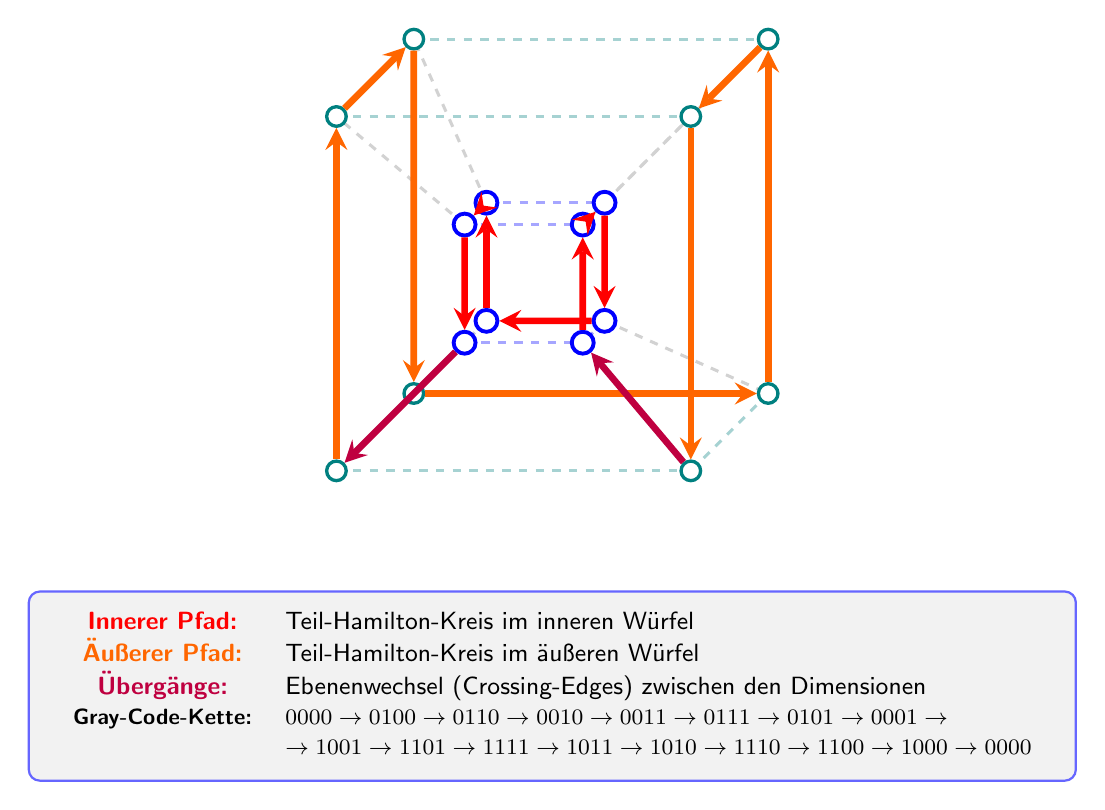
\begin{tikzpicture}[scale=1.5, thick, >=stealth]
  % \begin{ai-tikz-planner-invisible-content}
  % 1. Background: Projektion des Tesseracts (Q_4) mit strukturell getrennten Dimensionen. Der innere 3D-Würfel ist in Blau (blue) gezeichnet, der äußere in Teal (teal).
  % 2. Visual Hierarchy: Nicht-zyklische Kanten sind dünn, gestrichelt und farblich dezent gehalten (blue!35 bzw. teal!35).
  % 3. Foreground Layering & Shading: Ecken werden zuerst als benannte Kreise (n0000 bis n1111) gezeichnet. Der rote Pfad (Hamilton-Kreis / Gray-Code) wird danach im Vordergrund über die Ecken gelegt. Der Pfad ist farblich schattiert (red im inneren Würfel, orange!80!red im äußeren Würfel, purple für die Ebenen-Wechsel-Übergänge).
  % 4. Legend: Eine detaillierte Legende am Fuß der Grafik erklärt den Farbcode und den mathematisch korrekten 4-Bit Gray-Code.
  % \end{ai-tikz-planner-invisible-content}
  
  % Inner Cube Coordinates
  \coordinate (0000) at (-0.5,-0.5,-0.5);
  \coordinate (1000) at (0.5,-0.5,-0.5);
  \coordinate (1100) at (0.5,0.5,-0.5);
  \coordinate (0100) at (-0.5,0.5,-0.5);
  \coordinate (0010) at (-0.3,-0.3,0.5);
  \coordinate (1010) at (0.7,-0.3,0.5);
  \coordinate (1110) at (0.7,0.7,0.5);
  \coordinate (0110) at (-0.3,0.7,0.5);
  
  % Outer Cube Coordinates
  \coordinate (0001) at (-1.5,-1.5,-1.5);
  \coordinate (1001) at (1.5,-1.5,-1.5);
  \coordinate (1101) at (1.5,1.5,-1.5);
  \coordinate (0101) at (-1.5,1.5,-1.5);
  \coordinate (0011) at (-1.0,-1.0,1.5);
  \coordinate (1011) at (2.0,-1.0,1.5);
  \coordinate (1111) at (2.0,2.0,1.5);
  \coordinate (0111) at (-1.0,2.0,1.5);

  % 1. Non-cycle edges (dashed, thin)
  % Inner Cube (blue!35)
  \draw[blue!35, dashed, line width=1.1pt] (0000) -- (1000);
  \draw[blue!35, dashed, line width=1.1pt] (0100) -- (1100);
  \draw[blue!35, dashed, line width=1.1pt] (0010) -- (1010);
  \draw[blue!35, dashed, line width=1.1pt] (0110) -- (1110);
  \draw[blue!35, dashed, line width=1.1pt] (0000) -- (0010);
  \draw[blue!35, dashed, line width=1.1pt] (1000) -- (1010);
  
  % Outer Cube (teal!35)
  \draw[teal!35, dashed, line width=1.1pt] (0001) -- (1001);
  \draw[teal!35, dashed, line width=1.1pt] (0101) -- (1101);
  \draw[teal!35, dashed, line width=1.1pt] (0011) -- (1011);
  \draw[teal!35, dashed, line width=1.1pt] (0111) -- (1111);
  \draw[teal!35, dashed, line width=1.1pt] (0001) -- (0011);
  \draw[teal!35, dashed, line width=1.1pt] (1001) -- (1011);
  
  % Connecting Edges (gray!35)
  \draw[gray!35, dashed, line width=1.1pt] (0000) -- (0001);
  \draw[gray!35, dashed, line width=1.1pt] (1000) -- (1001);
  \draw[gray!35, dashed, line width=1.1pt] (1100) -- (1101);
  \draw[gray!35, dashed, line width=1.1pt] (0100) -- (0101);
  \draw[gray!35, dashed, line width=1.1pt] (1110) -- (1111);
  \draw[gray!35, dashed, line width=1.1pt] (0110) -- (0111);

  % 2. Vertices (Styled circles) - Drawn BEFORE the cycle paths
  % Outer Cube Ecken (teal)
  \foreach \p in {0001,1001,1101,0101,0011,1011,1111,0111}
    \node (n\p) [circle, draw=teal, fill=white, line width=1.2pt, inner sep=2.5pt] at (\p) {};
    
  % Inner Cube Ecken (blue)
  \foreach \p in {0000,1000,1100,0100,0010,1010,1110,0110}
    \node (n\p) [circle, draw=blue, fill=white, line width=1.4pt, inner sep=2.8pt] at (\p) {};

  % 3. Hamilton Cycle / Gray-Code Path in Foreground (Bold, colored by dimension/transition)
  % Inner Cube Path segments (red)
  \draw[->, red, line width=2.4pt] (n0000) -- (n0100);
  \draw[->, red, line width=2.4pt] (n0100) -- (n0110);
  \draw[->, red, line width=2.4pt] (n0110) -- (n0010);
  
  \draw[->, red, line width=2.4pt] (n1010) -- (n1110);
  \draw[->, red, line width=2.4pt] (n1110) -- (n1100);
  \draw[->, red, line width=2.4pt] (n1100) -- (n1000);
  \draw[->, red, line width=2.4pt] (n1000) -- (n0000);

  % Outer Cube Path segments (orange!80!red)
  \draw[->, orange!80!red, line width=2.4pt] (n0011) -- (n0111);
  \draw[->, orange!80!red, line width=2.4pt] (n0111) -- (n0101);
  \draw[->, orange!80!red, line width=2.4pt] (n0101) -- (n0001);
  \draw[->, orange!80!red, line width=2.4pt] (n0001) -- (n1001);
  \draw[->, orange!80!red, line width=2.4pt] (n1001) -- (n1101);
  \draw[->, orange!80!red, line width=2.4pt] (n1101) -- (n1111);
  \draw[->, orange!80!red, line width=2.4pt] (n1111) -- (n1011);

  % Crossing / Transition Path segments (purple)
  \draw[->, purple, line width=2.4pt] (n0010) -- (n0011);
  \draw[->, purple, line width=2.4pt] (n1011) -- (n1010);

  % 4. Explanatory Legend / Caption badge below
  \node[draw=blue!60, fill=gray!10, rounded corners=4pt, inner xsep=10pt, inner ysep=6pt, font=\sffamily\small] at (0.25, -3.4) {
    \begin{tabular}{cl}
      \textbf{\textcolor{red}{Innerer Pfad:}} & Teil-Hamilton-Kreis im inneren Würfel \\
      \textbf{\textcolor{orange!80!red}{Äußerer Pfad:}} & Teil-Hamilton-Kreis im äußeren Würfel \\
      \textbf{\textcolor{purple}{Übergänge:}} & Ebenenwechsel (Crossing-Edges) zwischen den Dimensionen \\
      \footnotesize \textbf{Gray-Code-Kette:} & \footnotesize $0000 \to 0100 \to 0110 \to 0010 \to 0011 \to 0111 \to 0101 \to 0001 \to {}$ \\
      & \footnotesize $\to 1001 \to 1101 \to 1111 \to 1011 \to 1010 \to 1110 \to 1100 \to 1000 \to 0000$
    \end{tabular}
  };
\end{tikzpicture}
\end{center}
\end{math-stroke}



\begin{spoken-clean}[00:54:38 - 00:56:52]
Solche Würfelstrukturen sind in vielen Bereichen der modernen Mathematik von großer Bedeutung. In der geometrischen Gruppentheorie war es in den letzten Jahren beispielsweise sehr populär, sogenannte kubische Komplexe zu untersuchen. Dabei nimmt man Würfel verschiedener Dimensionen, klebt sie nach bestimmten geometrischen Regeln zusammen und erhält dadurch mächtige Werkzeuge, um abstrakte Gruppen über die Kantengraphen dieser Komplexe zu studieren.

Das ist natürlich nicht Teil dieser Vorlesung, aber es war für einige Jahre mein persönliches Steckenpferd, diese kubischen Komplexe auf mathematische Gruppen anzuwenden.
\end{spoken-clean}

\section{Bipartite Graphen}

\begin{spoken-clean}[00:56:52 - 00:58:30]
Als letztes Thema für heute möchte ich mit Ihnen den sogenannten Heiratssatz besprechen --- auch wenn der Name historisch gesehen etwas unglücklich gewählt ist.

Zuvor benötigen wir noch eine Definition, die Ihnen auch auf dem Übungsblatt begegnen wird: Wann heißt ein Graph bipartit? Bipartit bedeutet anschaulich, dass man die Knotenmenge so in zwei disjunkte Teilmengen aufteilen kann, dass alle Kanten des Graphen ausschließlich zwischen diesen beiden Mengen verlaufen.

Formal heißt ein Graph bipartit, wenn sich die Knotenmenge $V$ als disjunkte Vereinigung zweier Teilmengen $U$ und $W$ schreiben lässt. Disjunkte Vereinigung bedeutet: $V = U \cup W$ und der Durchschnitt von $U$ und $W$ ist leer.
\end{spoken-clean}

\begin{math-stroke}
\begin{definition}[Bipartiter Graph]\label[definition]{def:bipartit}
Ein ungerichteter Graph $G = (V, E)$ heißt \newterm{bipartit}, falls sich seine Knotenmenge $V$ als disjunkte Vereinigung zweier Teilmengen $U$ und $W$ darstellen lässt:
\[
V = U \;\dot{\cup}\; W \quad (\text{d.\,h. } V = U \cup W \text{ und } U \cap W = \emptyset)
\]
sodass alle Kanten in $E$ ausschließlich zwischen $U$ und $W$ verlaufen:
\[
E \subseteq \bigl\{ \{u, w\} \;\big|\; u \in U, w \in W \bigr\}
\]
Wir schreiben einen solchen Graphen auch als Tripel $G = (U, W, E)$.
\end{definition}

\begin{center}
\begin{tikzpicture}[scale=1.2, thick, >=stealth]
  % \begin{ai-tikz-planner-invisible-content}
  % 1. Background: Bipartiter Graph mit zwei disjunkten Spalten U und W.
  % 2. Foreground: Kanten, die ausschließlich zwischen U und W verlaufen (keine internen Kanten).
  % \end{ai-tikz-planner-invisible-content}
  
  % Column U (ForestGreen)
  \coordinate (U1) at (0,2.5);
  \coordinate (U2) at (0,1.5);
  \coordinate (U3) at (0,0.5);
  
  % Column W (MidnightBlue)
  \coordinate (W1) at (3,2.5);
  \coordinate (W2) at (3,1.5);
  \coordinate (W3) at (3,0.5);
  
  % Edges
  \draw (U1) -- (W1);
  \draw (U1) -- (W2);
  \draw (U2) -- (W2);
  \draw (U2) -- (W3);
  \draw (U3) -- (W1);
  \draw (U3) -- (W3);
  
  % Nodes
  \filldraw[fill=white, draw=black] (U1) circle (3pt) node[left] {$u_1$};
  \filldraw[fill=white, draw=black] (U2) circle (3pt) node[left] {$u_2$};
  \filldraw[fill=white, draw=black] (U3) circle (3pt) node[left] {$u_3$};
  
  % Nodes (W)
  \filldraw[fill=white, draw=black] (W1) circle (3pt) node[right] {$w_1$};
  \filldraw[fill=white, draw=black] (W2) circle (3pt) node[right] {$w_2$};
  \filldraw[fill=white, draw=black] (W3) circle (3pt) node[right] {$w_3$};
  
  % Labels
  \node[above=0.3cm of U1, ForestGreen, font=\bfseries] {$U$};
  \node[above=0.3cm of W1, MidnightBlue, font=\bfseries] {$W$};
\end{tikzpicture}
\end{center}
\end{math-stroke}

\begin{spoken-clean}[00:58:30 - 00:59:56]
...sodass alle Kanten in der Menge $U \times W$ enthalten sind, was natürlich eine Teilmenge von $V \times V$ ist. Wir schreiben dann kurz: $G = (U, W, E)$.

Wenn wir also sagen, $G$ ist ein bipartiter Graph und schreiben ihn in dieser Form, dann bedeutet das: $U$ ist die eine Knotenmenge, $W$ die andere, und alle Kanten verlaufen ausschließlich zwischen Elementen aus $U$ und Elementen aus $W$.

Das ist eine sehr spezielle Struktur --- die meisten Graphen sind im Allgemeinen natürlich nicht bipartit.
\end{spoken-clean}

% --- TEIL 3 ---

\subsection{Bipartite Graphen und Färbbarkeit}

\begin{math-stroke}
\begin{theorem}[Zwei-Färbbarkeit bipartiter Graphen]\label[theorem]{thm:bipartit-faerbbarkeit}
Ein ungerichteter Graph $G = (V, E)$ ist genau dann bipartit, wenn er zwei-färbbar ist. Das bedeutet, es existiert eine Färbungsfunktion $c \colon V \to \{\text{Rot}, \text{Blau}\}$, sodass für alle Kanten $\{u, v\} \in E$ gilt:
\[
c(u) \neq c(v).
\]
\end{theorem}

\begin{explanation-of-steps}[Bedeutung der Zwei-Färbbarkeit]
In einem bipartiten Graphen $G = (U, W, E)$ können wir allen Knoten in $U$ die Farbe Rot und allen Knoten in $W$ die Farbe Blau zuweisen. Da per Definition alle Kanten ausschließlich zwischen $U$ und $W$ verlaufen, gibt es keine Kanten zwischen gleichfarbigen Knoten. Dies zeigt die Äquivalenz zur Zwei-Färbbarkeit.
\end{explanation-of-steps}
\end{math-stroke}

\begin{spoken-clean}[00:59:56 - 01:01:08]
Bipartite Graphen treten in der Praxis erstaunlich häufig auf. Denken Sie beispielsweise an ein Netzwerk von Brieffreundschaften zwischen Menschen in Europa und Menschen in Amerika: Jede Person lebt entweder in Europa oder in Amerika, und Briefe werden definitionsgemäß nur über den Atlantik hinweg ausgetauscht. Das ist ein klassischer bipartiter Graph.
\end{spoken-clean}

\begin{math-stroke}[Beispiel eines bipartiten Graphen]
\begin{example}[Brieffreunde-Netzwerk]\label[example]{ex:brieffreunde}
Betrachte das Netzwerk von Brieffreunden zwischen Europa und Amerika. Wir definieren den Graphen $G = (U, W, E)$ durch:
\begin{itemize}
    \item \textbf{$U$:} Die Menge der Personen in Europa.
    \item \textbf{$W$:} Die Menge der Personen in Amerika.
    \item \textbf{$E$:} Die Menge der Kanten, wobei $\{u, w\} \in E$ bedeutet, dass $u \in U$ und $w \in W$ Brieffreunde sind.
\end{itemize}
Da Briefe nur über den Atlantik geschickt werden (keine Brieffreundschaften innerhalb Europas oder innerhalb Amerikas), ist dieser Graph bipartit.
\end{example}
\end{math-stroke}

\begin{spoken-clean}[01:01:08 - 01:02:13]
Machen wir noch eine Definition für ungerichtete bipartite Graphen. Bei bipartiten Graphen spielt die Unterscheidung zwischen gerichtet und ungerichtet ohnehin keine allzu große Rolle, da man für jede Kante durch die Aufteilung der Knotenmengen immer genau weiß, ob sie in $U$ beginnt und in $W$ endet.
\end{spoken-clean}

\begin{math-stroke}
\begin{definition}[Bipartiter Graph]\label[definition]{def:bipartit-formal}
Ein ungerichteter Graph $G = (V, E)$ heißt \newterm{bipartit}, falls sich seine Knotenmenge $V$ als disjunkte Vereinigung zweier Teilmengen $U$ und $W$ darstellen lässt:
\[
V = U \;\dot{\cup}\; W \quad (\text{d.\,h. } V = U \cup W \text{ und } U \cap W = \emptyset),
\]
sodass alle Kanten in $E$ ausschließlich zwischen $U$ und $W$ verlaufen:
\[
E \subseteq \bigl\{ \{u, w\} \;\big|\; u \in U, w \in W \bigr\}.
\]
Wir schreiben einen solchen Graphen auch als Tripel $G = (U, W, E)$.
\end{definition}
\end{math-stroke}

\begin{spoken-clean}[01:02:13 - 01:03:23]
Wir definieren nun für eine Teilmenge $X \subseteq U$ die Nachbarschaft $E(X)$ als die Menge aller Knoten $y \in W$, für die ein $x \in X$ existiert, sodass $\{x, y\}$ eine Kante im Graphen ist. Analog definieren wir die Nachbarschaft $E(Y)$ für eine Teilmenge $Y \subseteq W$.
\end{spoken-clean}

\begin{ai-global-state-checkpoint-invisible-content}
% timestamp: 01:03:23
% topic: Definition der Nachbarschaft in bipartiten Graphen
% board_state: def:bipartit-formal, def:nachbarschaft-bipartit
% next_goal: Visualisierung der Nachbarschaft und Einführung des Heiratssatzes
% open_loops: none
\end{ai-global-state-checkpoint-invisible-content}

\begin{math-stroke}
\begin{definition}[Nachbarschaft]\label[definition]{def:nachbarschaft-bipartit}
Sei $G = (U, W, E)$ ein bipartiter Graph. Für eine Teilmenge von Knoten $X \subseteq U$ definieren wir die \newterm{Nachbarschaft} $E(X)$ (oft auch als $N(X)$ bezeichnet) als die Menge aller Knoten in $W$, die mit mindestens einem Knoten aus $X$ verbunden sind:
\[
E(X) := \bigl\{ y \in W \;\big|\; \exists x \in X \colon \{x, y\} \in E \bigr\}.
\]
Analog definieren wir die Nachbarschaft $E(Y)$ für eine Teilmenge $Y \subseteq W$.
\end{definition}
\end{math-stroke}

\begin{spoken-clean}[01:03:23 - 01:04:39]
Anschaulich bedeutet das: Auf der einen Seite haben wir die Knotenmenge $U$, auf der anderen Seite die Knotenmenge $W$, und dazwischen verlaufen die Kanten. Wenn wir nun eine Teilmenge $X \subseteq U$ betrachten, dann ist $E(X)$ die Menge all derjenigen Knoten in $W$, die mit mindestens einem Knoten aus $X$ durch eine Kante verbunden sind.
\end{spoken-clean}

\begin{math-stroke}[Visualisierung der Nachbarschaft]
\begin{center}
\begin{tikzpicture}[scale=1.3, thick, >=stealth]
  % \begin{ai-tikz-planner-invisible-content}
  % 1. Background: Bipartiter Graph mit zwei disjunkten Spalten U und W.
  % 2. Midground: Teilmenge X in U (lila hinterlegt) und ihre Nachbarschaft E(X) in W (orange hinterlegt).
  % 3. Foreground: Kanten, die von X nach E(X) verlaufen.
  % \end{ai-tikz-planner-invisible-content}
  
  % Column U
  \coordinate (U1) at (0,3);
  \coordinate (U2) at (0,2);
  \coordinate (U3) at (0,1);
  \coordinate (U4) at (0,0);
  
  % Column W
  \coordinate (W1) at (4,3);
  \coordinate (W2) at (4,2);
  \coordinate (W3) at (4,1);
  \coordinate (W4) at (4,0);
  
  % Shading for X (lila)
  \draw[fill=Fuchsia!10, draw=Fuchsia, dashed, rounded corners=5pt] (-0.4, 0.6) rectangle (0.4, 2.4);
  \node[Fuchsia, left=0.5cm of U2] {\textbf{$X$}};
  
  % Shading for E(X) (orange)
  \draw[fill=BurntOrange!10, draw=BurntOrange, dashed, rounded corners=5pt] (3.6, 0.6) rectangle (4.4, 3.4);
  \node[BurntOrange, right=0.5cm of W2] {\textbf{$E(X)$}};
  
  % Edges
  \draw[thick, Fuchsia] (U2) -- (W1);
  \draw[thick, Fuchsia] (U2) -- (W2);
  \draw[thick, Fuchsia] (U3) -- (W2);
  \draw[thick, Fuchsia] (U3) -- (W3);
  \draw[thick, gray!40] (U1) -- (W1);
  \draw[thick, gray!40] (U4) -- (W4);
  
  % Nodes
  \filldraw[fill=white, draw=black] (U1) circle (3pt) node[left] {$u_1$};
  \filldraw[fill=white, draw=black] (U2) circle (3pt) node[left] {$u_2$};
  \filldraw[fill=white, draw=black] (U3) circle (3pt) node[left] {$u_3$};
  \filldraw[fill=white, draw=black] (U4) circle (3pt) node[left] {$u_4$};
  
  % Nodes (W)
  \filldraw[fill=white, draw=black] (W1) circle (3pt) node[right] {$w_1$};
  \filldraw[fill=white, draw=black] (W2) circle (3pt) node[right] {$w_2$};
  \filldraw[fill=white, draw=black] (W3) circle (3pt) node[right] {$w_3$};
  \filldraw[fill=white, draw=black] (W4) circle (3pt) node[right] {$w_4$};
  
  % Labels
  \node[above=0.4cm of U1, ForestGreen, font=\bfseries] {$U$};
  \node[above=0.35cm of W1, MidnightBlue, font=\bfseries] {$W$};
\end{tikzpicture}
\end{center}
\end{math-stroke}

\section{Der Heiratssatz von Hall}

\begin{spoken-clean}[01:04:39 - 01:05:58]
Es geht dabei um folgendes Problem, das ich Ihnen kurz erklären möchte. Ich werde gar nicht erst versuchen zu begründen, weshalb dieses Resultat historisch 'Heiratssatz' genannt wurde --- denn diese Namensgebung beruht auf völlig veralteten, heteronormativen und binären Vorstellungen, die wir hier gar nicht weiter betrachten wollen. Der Satz stammt schließlich aus den 1950er Jahren.
\end{spoken-clean}

\begin{spoken-clean}[01:05:58 - 01:07:08]
Das mathematische Problem lässt sich aber sehr anschaulich erklären. Stellen wir uns vor, wir haben eine Gruppe von Personen, beispielsweise $A, B, C, D, E$, und eine Menge von Geschenken oder Objekten, die diese Personen gerne hätten. Jede Person hat bestimmte Präferenzen: $A$ möchte zum Beispiel das Geschenk $1$ oder $3$, $B$ hätte gerne $2, 4, 5$ oder $6$, $C$ bevorzugt $2$ oder $3$, $D$ möchte $1$, und so weiter. Solche Situationen kennt man ja vom Kindergeburtstag, wo jedes Kind sich ein Geschenk aus einem Korb aussuchen darf und jeder eine persönliche Wunschliste im Kopf hat.
\end{spoken-clean}

\begin{math-stroke}[Beispiel zum Heiratssatz]
\begin{center}
\begin{tikzpicture}[scale=1.3, thick, >=stealth]
  % \begin{ai-tikz-planner-invisible-content}
  % 1. Background: Bipartiter Graph mit Personen A, B, C, D, E auf der linken Seite und Geschenken 1, 2, 3, 4, 5, 6 auf der rechten Seite.
  % 2. Foreground: Präferenzkanten zwischen Personen und Geschenken.
  % \end{ai-tikz-planner-invisible-content}
  
  % Left Column: Personen (A, B, C, D, E)
  \coordinate (A) at (0,4);
  \coordinate (B) at (0,3);
  \coordinate (C) at (0,2);
  \coordinate (D) at (0,1);
  \coordinate (E) at (0,0);
  
  % Right Column: Geschenke (1, 2, 3, 4, 5, 6)
  \coordinate (G1) at (4,4.5);
  \coordinate (G2) at (4,3.6);
  \coordinate (G3) at (4,2.7);
  \coordinate (G4) at (4,1.8);
  \coordinate (G5) at (4,0.9);
  \coordinate (G6) at (4,0);
  
  % Edges (Preferences)
  \draw (A) -- (G1);
  \draw (A) -- (G3);
  \draw (B) -- (G2);
  \draw (B) -- (G4);
  \draw (B) -- (G5);
  \draw (B) -- (G6);
  \draw (C) -- (G2);
  \draw (C) -- (G3);
  \draw (D) -- (G1);
  \draw (D) -- (G4);
  \draw (E) -- (G5);
  
  % Nodes (Personen)
  \filldraw[fill=white, draw=black] (A) circle (3pt) node[left] {$A$};
  \filldraw[fill=white, draw=black] (B) circle (3pt) node[left] {$B$};
  \filldraw[fill=white, draw=black] (C) circle (3pt) node[left] {$C$};
  \filldraw[fill=white, draw=black] (D) circle (3pt) node[left] {$D$};
  \filldraw[fill=white, draw=black] (E) circle (3pt) node[left] {$E$};
  
  % Nodes (Geschenke)
  \filldraw[fill=white, draw=black] (G1) circle (3pt) node[right] {$1$};
  \filldraw[fill=white, draw=black] (G2) circle (3pt) node[right] {$2$};
  \filldraw[fill=white, draw=black] (G3) circle (3pt) node[right] {$3$};
  \filldraw[fill=white, draw=black] (G4) circle (3pt) node[right] {$4$};
  \filldraw[fill=white, draw=black] (G5) circle (3pt) node[right] {$5$};
  \filldraw[fill=white, draw=black] (G6) circle (3pt) node[right] {$6$};
  
  % Labels
  \node[above=0.3cm of A, ForestGreen, font=\bfseries] {Personen};
  \node[above=0.3cm of G1, MidnightBlue, font=\bfseries] {Geschenke};
\end{tikzpicture}
\end{center}
\end{math-stroke}

\begin{spoken-clean}[01:07:08 - 01:08:20]
Gibt es nun eine Möglichkeit, die Geschenke so zu verteilen, dass am Ende jede Person ein Objekt erhält, das auf ihrer Wunschliste steht? Mathematisch formuliert lautet die Frage: Gibt es eine injektive Abbildung von der Personenmenge in die Objektmenge, bei der wir jeder Person ein Element zuordnen, das mit ihr durch eine Kante verbunden ist? Das ist ein sehr klassisches und praktisches Verteilungsproblem.
\end{spoken-clean}

\begin{spoken-clean}[01:08:20 - 01:09:40]
Das betrifft nicht nur Kindergeburtstage, sondern kann in vielen realen Szenarien eine Rolle spielen --- beispielsweise bei der Zuteilung von Masterarbeitsplätzen an Studierende. Die zentrale Frage lautet: Unter welchen Bedingungen besitzt dieses Problem für einen gegebenen Graphen eine Lösung? Wann existiert eine solche Injektion? Der Heiratssatz liefert uns hierfür eine präzise notwendige und hinreichende Bedingung. Denn wenn beispielsweise alle Personen dasselbe einzige Objekt wollen, kann es offensichtlich keine Lösung geben.
\end{spoken-clean}

\begin{ai-global-state-checkpoint-invisible-content}
% timestamp: 01:07:18
% topic: Einführung des Heiratssatzes von Hall
% board_state: def:nachbarschaft-bipartit, ex:platonische-koerper
% next_goal: Formulierung des Heiratssatzes (Hall)
% open_loops: none
\end{ai-global-state-checkpoint-invisible-content}

\begin{spoken-clean}[01:09:40 - 01:11:00]
Der Heiratssatz --- formuliert von dem Gruppentheoretiker Philip Hall --- gibt uns hierauf die Antwort. Wir schreiben das einmal formal auf: Sei $G = (A, B, E)$ ein endlicher, ungerichteter, bipartiter Graph. Dann sind die folgenden Aussagen äquivalent: \textbf{(a)} Es existiert eine Injektion $\pi \colon A \to B$, sodass für alle $a \in A$ gilt, dass $\{a, \pi(a)\}$ eine Kante ist. Und \textbf{(b)} für alle Teilmengen $X \subseteq A$ gilt die Hall-Bedingung: $|X| \le |E(X)|$.
\end{spoken-clean}

\begin{math-stroke}
\begin{theorem}[Heiratssatz von Hall]\label[theorem]{thm:heiratssatz}
Sei $G = (A, B, E)$ ein endlicher, ungerichteter, bipartiter Graph. Dann sind die folgenden Aussagen äquivalent:
\begin{enumerate}[label=\textbf{(\alph*)}]
    \item Es existiert eine Injektion $\pi \colon A \to B$, sodass für alle $a \in A$ gilt:
    \[
    \{a, \pi(a)\} \in E.
    \]
    \item Für alle Teilmengen $X \subseteq A$ gilt die Hall-Bedingung:
    \[
    |X| \le |E(X)|.
    \]
\end{enumerate}
\end{theorem}

\begin{explanation-of-steps}[Interpretation der Hall-Bedingung]
Die Bedingung \textbf{(b)} besagt anschaulich, dass jede Gruppe von Personen $X \subseteq A$ insgesamt mindestens so viele verschiedene Geschenke (bzw. Partner) in $B$ bevorzugen muss, wie es Personen in der Gruppe gibt. Ist diese Bedingung für auch nur eine einzige Teilmenge verletzt (d.\,h. $|X| > |E(X)|$), so können offensichtlich nicht alle Personen aus $X$ gleichzeitig ein bevorzugtes Geschenk erhalten. Hall zeigte, dass diese offensichtlich notwendige Bedingung auch hinreichend ist.
\end{explanation-of-steps}
\end{math-stroke}

\begin{spoken-clean}[01:11:00 - 01:12:30]
Manche Autoren verwenden zur Veranschaulichung diese Begrifflichkeiten: Zwei Elemente $a$ und $b$ heißen befreundet, wenn zwischen ihnen eine Kante existiert, und eine solche injektive Abbildung $\pi$ wird dann als Heiratsfunktion bezeichnet. Die Frage lautet also, ob man alle Elemente aus $A$ monogam mit Elementen aus $B$ verheiraten kann, sodass nur befreundete Paare entstehen. Diese Bedingung ist sowohl notwendig als auch hinreichend.
\end{spoken-clean}

\begin{math-stroke}
\begin{definition}[Heiratsfunktion / Matching]\label[definition]{def:matching}
Sei $G = (A, B, E)$ ein bipartiter Graph.
\begin{itemize}
    \item Eine Kante $\{a, b\} \in E$ repräsentiert eine \newterm{Freundschaft} zwischen $a \in A$ und $b \in B$.
    \item Eine Injektion $\pi \colon A \to B$ mit $\{a, \pi(a)\} \in E$ für alle $a \in A$ heißt eine \newterm{Heiratsfunktion} (oder ein \newterm{vollständiges Matching} von $A$ nach $B$).
\end{itemize}
\end{definition}
\end{math-stroke}

\subsection{Beweis des Heiratssatzes}

\begin{proof}[Beweis des Heiratssatzes von Hall]
\begin{spoken-clean}[01:12:30 - 01:14:50]
Wir nehmen an, es existiert eine Heiratsfunktion $\pi \colon A \to B$. Sei $X \subseteq A$ eine beliebige Teilmenge. Da $\pi$ eine Injektion ist, gilt für die Mächtigkeit des Bildes von $X$: $|X| = |\pi(X)|$. Da für jedes $x \in X$ gilt, dass $\{x, \pi(x)\} \in E$ ist, liegt das Bild von $X$ per Definition vollständig in der Nachbarschaft von $X$: $\pi(X) \subseteq E(X)$. Daraus folgt unmittelbar für die Mächtigkeiten: $|X| = |\pi(X)| \le |E(X)|$. Dies zeigt, dass die Hall-Bedingung \textbf{(b)} eine notwendige Bedingung für die Existenz einer Heiratsfunktion ist.
\end{spoken-clean}

\begin{ai-global-state-checkpoint-invisible-content}
% timestamp: 01:12:31
% topic: Beweis des Heiratssatzes (Hinrichtung)
% board_state: thm:heiratssatz, def:matching
% next_goal: Induktionsbeweis der Rückrichtung (b) => (a)
% open_loops: none
\end{ai-global-state-checkpoint-invisible-content}

\begin{math-stroke}
\textbf{Hinrichtung (\texorpdfstring{\textbf{(a)} $\implies$ \textbf{(b)}}{a -> b}):}
Wir nehmen an, es existiert eine Heiratsfunktion $\pi \colon A \to B$. Sei $X \subseteq A$ eine beliebige Teilmenge.
        
Da $\pi$ eine Injektion ist, gilt für die Mächtigkeit des Bildes von $X$:
\[
|X| = |\pi(X)|.
\]
Da für jedes $x \in X$ gilt, dass $\{x, \pi(x)\} \in E$ ist, liegt das Bild von $X$ per Definition vollständig in der Nachbarschaft von $X$:
\[
\pi(X) \subseteq E(X).
\]
Daraus folgt unmittelbar für die Mächtigkeiten:
\[
|X| = |\pi(X)| \le |E(X)|.
\]
Dies zeigt, dass die Hall-Bedingung \textbf{(b)} eine notwendige Bedingung für die Existenz einer Heiratsfunktion ist.
\end{math-stroke}

\begin{spoken-clean}[01:14:50 - 01:16:15]
Es ist klar, dass wenn so eine Heiratsfunktion existiert, dann muss diese Bedingung erfüllt sein. Ansonsten... ja, sonst geht's nicht. Jetzt das, was eigentlich der wichtige Satz ist, ist, dass das auch hinreichend ist. Also wenn diese Bedingung erfüllt ist, dann gibt es eine solche Funktion. Okay, und jetzt um zu zeigen, dass (b) impliziert (a)... Da machen wir jetzt Induktion, und zwar nach der Anzahl Elemente in $A$.
\end{spoken-clean}

\begin{spoken-clean}[01:16:15 - 01:17:20]
Wir nehmen jetzt an, (b) ist erfüllt, und wir machen jetzt Induktion über die Anzahl Elemente von $A$ und zeigen, dass es jeweils so eine... so eine Funktion gibt. Okay, also falls $n = 1$ ist, ist der Fall klar. Ich meine, wenn es nur ein Element hat in $A$, okay, dann muss es mindestens eine Kante geben, die von $A$ weggeht. Wenn es das gibt, dann gibt es eine solche Funktion. Okay, also wenn das erfüllt ist, dann gibt es mindestens eine Kante, das heißt es gibt auch eine Funktion.
\end{spoken-clean}

\begin{spoken-clean}[01:17:20 - 01:18:30]
Das heißt, wir müssen nun den Induktionsschritt von $n$ auf $n+1$ vollziehen. Wir nehmen also an, die Behauptung sei für alle Graphen bewiesen, bei denen die Knotenmenge $A$ höchstens $n$ Elemente enthält. Nun müssen wir den Satz für $n+1$ beweisen.
\end{spoken-clean}

\begin{spoken-clean}[01:18:30 - 01:20:00]
Dazu betrachten wir zwei Fälle. Der erste Fall ist dadurch charakterisiert, dass für alle echten Teilmengen $X \subsetneq A$ die Mächtigkeit $|X|$ nicht nur kleiner gleich $|E(X)|$ ist --- was wir ohnehin durch die Hall-Bedingung wissen ---, sondern sogar strikt kleiner ist: $|X| < |E(X)|$. Die Voraussetzung gibt uns also $|X| \le |E(X)|$, aber im ersten Fall nehmen wir an, dass für jede echte Teilmenge sogar die strikte Ungleichung gilt.
\end{spoken-clean}

\begin{spoken-clean}[01:20:00 - 01:21:30]
In diesem Fall wählen wir eine beliebige Kante $\{a', b'\} \in E$. Wir definieren nun die reduzierten Mengen $A' := A \setminus \{a'\}$ und $B' := B \setminus \{b'\}$.
\end{spoken-clean}

\begin{ai-global-state-checkpoint-invisible-content}
% timestamp: 01:17:43
% topic: Induktionsbeweis des Heiratssatzes (Fallunterscheidung)
% board_state: thm:heiratssatz, proof:euler-forward
% next_goal: Beweis von Fall 1 (Strikte Ungleichung)
% open_loops: none
\end{ai-global-state-checkpoint-invisible-content}

\begin{spoken-clean}[01:21:30 - 01:22:50]
Nun betrachten wir die verbleibenden Kanten zwischen diesen beiden Mengen. Wir definieren $E'$ als die Menge der Kanten, die von $A'$ nach $B'$ verlaufen --- also alle ursprünglichen Kanten aus $E$ ohne diejenigen, die an $a'$ oder $b'$ angrenzen.
\end{spoken-clean}

\begin{spoken-clean}[01:22:50 - 01:24:30]
Für jede Teilmenge $X \subseteq A'$ gilt nach unserer Annahme $|X| < |E(X)|$. Da es sich um ganze Zahlen handelt, folgt daraus $|X| \le |E(X)| - 1$. Dies ist wiederum kleiner gleich der Mächtigkeit von $E(X) \setminus \{b'\}$. Wir betrachten also alle Nachbarn von $X$ in $B$, ziehen aber eventuell den Knoten $b'$ ab. Das ist aber genau die Nachbarschaft $E'(X)$ im reduzierten Graphen --- also alle Nachbarn von $X$, die in $B'$ liegen.
\end{spoken-clean}

\begin{spoken-clean}[01:24:30 - 01:26:00]
Das bedeutet, dass die Hall-Bedingung auch für den reduzierten Graphen $G' = (A', B', E')$ erfüllt ist. Da $|A'| = n$ ist, folgt nach der Induktionsvoraussetzung, dass eine injektive Heiratsfunktion $\pi' \colon A' \to B'$ existiert.
\end{spoken-clean}

\begin{spoken-clean}[01:26:00 - 01:27:20]
Für diese gilt natürlich $\{a, \pi'(a)\} \in E'$ für alle $a \in A'$. Nun können wir diese Abbildung zu einer Funktion $\pi \colon A \to B$ für den gesamten Graphen erweitern. Wir definieren einfach: $\pi(a) := b'$, falls $a = a'$ ist, und $\pi(a) := \pi'(a)$ andernfalls. Diese Abbildung ist injektiv und erfüllt die gewünschte Kantenbedingung aus \textbf{(a)}.
\end{spoken-clean}

\begin{ai-global-state-checkpoint-invisible-content}
% timestamp: 01:23:55
% topic: Abschluss des Beweises für Fall 1
% board_state: thm:heiratssatz, proof:euler-forward
% next_goal: Zusammenfassung und Abschluss der Vorlesung
% open_loops: none
\end{ai-global-state-checkpoint-invisible-content}

\begin{spoken-clean}[01:27:20 - 01:28:40]
Das beendet den Beweis für diesen ersten Fall. Schauen Sie sich den Beweis zu Hause noch einmal in Ruhe an --- er ist nicht allzu schwer, aber mathematisch äußerst elegant, wie hier alles perfekt aufgeht. Ein wirklich schöner Induktionsbeweis mit einer klugen Fallunterscheidung. Dem Heiratssatz werden Sie in der diskreten Mathematik immer wieder begegnen; es ist ein sehr berühmtes Resultat mit vielen verschiedenen Beweisvarianten. Wenn Sie im Internet danach suchen, finden Sie im Handumdrehen ein Dutzend unterschiedliche Zugänge. Gut, so weit für heute zur Graphentheorie.
\end{spoken-clean}

\begin{math-stroke}
\textbf{Rückrichtung (\texorpdfstring{\textbf{(b)} $\implies$ \textbf{(a)}}{b -> a}):}
Wir beweisen die Aussage mittels vollständiger Induktion nach $n := |A|$.
        
\textbf{Induktionsanfang ($n = 1$):} \\
Sei $A = \{a'\}$. Da $\emptyset \neq A \subseteq A$, gilt nach der Hall-Bedingung \textbf{(b)}:
\[
1 = |A| \le |E(A)| \implies E(A) \neq \emptyset.
\]
Es existiert also mindestens ein Element $b' \in B$ mit $\{a', b'\} \in E$. Wir definieren die Abbildung $\pi \colon A \to B$ durch $\pi(a') := b'$. Diese Abbildung ist trivialerweise injektiv und erfüllt $\{a', \pi(a')\} \in E$.
        
\textbf{Induktionsschritt ($n \to n+1$):} \\
Wir nehmen an, die Behauptung gilt für alle bipartiten Graphen mit $|A| \le n$. Sei nun $G = (A, B, E)$ ein bipartiter Graph mit $|A| = n+1$, der die Hall-Bedingung \textbf{(b)} erfüllt. Wir unterscheiden zwei Fälle:
        
\textbf{Fall 1: Für alle echten Teilmengen $\emptyset \neq X \subsetneq A$ gilt die strikte Ungleichung $|X| < |E(X)|$.}
\begin{enumerate}[label=\textbf{(\arabic*)}]
    \item \textbf{Wahl einer Kante:} Wir wählen eine beliebige Kante $\{a', b'\} \in E$ mit $a' \in A$ und $b' \in B$.
    \item \textbf{Konstruktion des reduzierten Graphen:} Wir definieren die reduzierten Mengen:
    \[
    A' := A \setminus \{a'\}, \quad B' := B \setminus \{b'\}
    \]
    sowie die eingeschränkte Kantenmenge $E' := E \cap (A' \times B')$. Der reduzierte Graph ist $G' = (A', B', E')$ mit $|A'| = n$.
    \item \textbf{Verifikation der Hall-Bedingung für $G'$:} Sei $X \subseteq A'$ eine beliebige Teilmenge.
    \begin{itemize}
        \item Falls $X = \emptyset$, gilt trivialerweise $|X| = 0 \le |E'(X)|$.
        \item Falls $X \neq \emptyset$, ist $X \subsetneq A$ eine echte Teilmenge von $A$ (da $a' \notin X$). Nach der Annahme von Fall 1 gilt:
        \[
        |X| < |E(X)| \implies |X| \le |E(X)| - 1.
        \]
        Da $b'$ das einzige Element ist, das in $B$ aber nicht in $B'$ liegt, gilt für die Nachbarschaft $E'(X)$ von $X$ im reduzierten Graphen $G'$:
        \[
        |E'(X)| \ge |E(X) \setminus \{b'\}| \ge |E(X)| - 1 \ge |X|.
        \]
        Somit erfüllt der reduzierte Graph $G'$ ebenfalls die Hall-Bedingung.
    \end{itemize}
    \item \textbf{Anwendung der Induktionsvoraussetzung:} Da $|A'| = n$, existiert nach Induktionsannahme eine Injektion $\pi' \colon A' \to B'$ mit $\{a, \pi'(a)\} \in E'$ für alle $a \in A'$.
    \item \textbf{Konstruktion der Gesamtinjektion:} Wir definieren $\pi \colon A \to B$ durch:
    \[
    \pi(a) := \begin{cases}
    b' & \text{falls } a = a' \\
    \pi'(a) & \text{falls } a \neq a'
    \end{cases}
    \]
    Da $\pi'$ injektiv ist und ihr Bild vollständig in $B'$ liegt (somit $b' \notin \operatorname{Im}(\pi')$), ist auch $\pi$ eine injektive Abbildung. Zudem gilt nach Konstruktion $\{a, \pi(a)\} \in E$ für alle $a \in A$.
\end{enumerate}
        
\textbf{Fall 2: Es existiert eine echte Teilmenge $\emptyset \neq A_1 \subsetneq A$ mit $|A_1| = |E(A_1)|$.}
\begin{enumerate}[label=\textbf{(\arabic*)}]
    \item \textbf{Aufteilung des Graphen:} Wir definieren $B_1 := E(A_1)$ und betrachten den Teilgraphen $G_1 = (A_1, B_1, E_1)$ mit $E_1 := E \cap (A_1 \times B_1)$. Da $|A_1| \le n$ und $G_1$ die Hall-Bedingung erbt, existiert nach Induktionsannahme eine Injektion $\pi_1 \colon A_1 \to B_1$ mit $\{a, \pi_1(a)\} \in E_1$ für alle $a \in A_1$. Da $|A_1| = |B_1|$, ist $\pi_1$ sogar eine Bijektion.
    \item \textbf{Betrachtung des Komplements:} Wir definieren die Komplementärmengen:
    \[
    A_2 := A \setminus A_1, \quad B_2 := B \setminus B_1
    \]
    und den Graphen $G_2 = (A_2, B_2, E_2)$ mit $E_2 := E \cap (A_2 \times B_2)$.
    \item \textbf{Verifikation der Hall-Bedingung für $G_2$:} Sei $X \subseteq A_2$ eine beliebige Teilmenge. Wir müssen zeigen, dass $|X| \le |E_2(X)|$ gilt.
    Betrachte die Vereinigung $X \cup A_1 \subseteq A$. Da $G$ die Hall-Bedingung erfüllt, gilt:
    \[
    |X \cup A_1| \le |E(X \cup A_1)| = |E(X) \cup E(A_1)|.
    \]
    Da $X$ und $A_1$ disjunkt sind, gilt $|X \cup A_1| = |X| + |A_1\|$. Zudem lässt sich die Nachbarschaft aufteilen in:
    \[
    E(X) \cup E(A_1) = E_2(X) \;\dot{\cup}\; E(A_1) = E_2(X) \;\dot{\cup}\; B_1.
    \]
    Daraus folgt für die Mächtigkeiten:
    \[
    |X| + |A_1| \le |E_2(X)| + |B_1|.
    \]
    Da nach Voraussetzung dieses Falles $|A_1| = |B_1|$ gilt, kürzen sich diese Terme weg und wir erhalten:
    \[
    |X| \le |E_2(X)|.
    \]
    Somit erfüllt auch $G_2$ die Hall-Bedingung.
    \item \textbf{Zusammenführung der Teillösungen:} Da $|A_2| < |A| = n+1$, existiert nach Induktionsannahme eine Injektion $\pi_2 \colon A_2 \to B_2$ mit $\{a, \pi_2(a)\} \in E_2$ für alle $a \in A_2$.
    Wir definieren die Gesamtinjektion $\pi \colon A \to B$ durch:
    \[
    \pi(a) := \begin{cases}
    \pi_1(a) & \text{falls } a \in A_1 \\
    \pi_2(a) & \text{falls } a \in A_2
    \end{cases}
    \]
    Da $\pi_1 \colon A_1 \to B_1$ und $\pi_2 \colon A_2 \to B_2$ injektiv sind und ihre Bildmengen $B_1$ und $B_2$ disjunkt sind, ist $\pi$ eine wohldefinierte Injektion auf ganz $A$, die die Kantenbedingung erfüllt.
\end{enumerate}
Dies schließt den Induktionsbeweis für beide Fälle ab.
\end{math-stroke}
\end{proof}

\begin{nice-box}[Zusammenfassung der Schlüsselkonzepte]
In dieser Vorlesung haben wir wichtige Grundlagen der Graphentheorie und deren praktische Anwendungen kennengelernt:
\begin{itemize}
    \item \textbf{Handschlaglemma:} Die Summe aller Knotengrade in einem Graphen ist stets doppelt so groß wie die Anzahl der Kanten ($\sum \deg(v) = 2|E|$). Daraus folgt, dass die Anzahl der Knoten mit ungeradem Grad immer gerade sein muss.
    \item \textbf{Euler-Linien und Euler-Graphen:} Ein zusammenhängender Graph besitzt genau dann eine geschlossene Euler-Linie (einen geschlossenen Kantenzug, der jede Kante exakt einmal enthält), wenn jeder Knotengrad gerade ist. Dies löst unter anderem das historische Königsberger Brückenproblem und das Dominoproblem.
    \item \textbf{Hamilton-Kreise und Hamilton-Graphen:} Ein Hamilton-Kreis ist ein geschlossener Weg, der jeden Knoten des Graphen genau einmal besucht. Im Gegensatz zu Euler-Graphen ist die Bestimmung der Hamiltonizität im Allgemeinen ein NP-schweres Problem. Wichtige Beispiele sind die Kantengraphen platonischer Körper und Hyperwürfel (deren Hamilton-Kreise den Gray-Codes entsprechen).
    \item \textbf{Bipartite Graphen:} Ein Graph ist bipartit, wenn sich seine Knotenmenge in zwei disjunkte Teilmengen $U$ und $W$ aufteilen lässt, sodass Kanten nur zwischen $U$ und $W$ verlaufen. Dies ist äquivalent zur Zwei-Färbbarkeit des Graphen.
    \item \textbf{Heiratssatz von Hall:} Ein bipartiter Graph $G = (A, B, E)$ besitzt genau dann ein vollständiges Matching (eine Heiratsfunktion) von $A$ nach $B$, wenn für jede Teilmenge $X \subseteq A$ die Hall-Bedingung $|X| \le |E(X)|$ erfüllt ist.
\end{itemize}
\end{nice-box}